\documentclass[a4paper,11pt]{jreport}
\usepackage{masterthesis}
\usepackage[dvipdfmx]{graphicx}
\usepackage{url}
\graphicspath{ {./figure/} }

%次の行を有効にすると、その章だけが読み込まれる
%\includeonly{introduction}

%----------------------------------------------------------------------
% タイトルページ
%----------------------------------------------------------------------
% タイトル 2行にわたる場合は適宜改行をいれること。
\title{拡張現実感を用いた看板画像からの\\店舗情報アクセス手法に関する研究}

% 提出年月
\date{平成 31 年 2 月}

% 執筆者
\author{北村 茂生}
%----------------------------------------------------------------------

\includeonly{introduction,design_guidline}

\begin{document}

%タイトルページ
\maketitle

\pagenumbering{roman}
\begin{abstract}

\end{abstract}

%目次
\tableofcontents

%----------------------------------------------------------------------
%本文
%----------------------------------------------------------------------
\newpage
\pagenumbering{arabic}

\chapter{序論}
\label{chapter:introduction}

本章では、本研究の実施に至った背景を説明し、対象とする課題を明確にする。

%------------------------------------------------------------------------
\section{本研究の背景}
\label{section:background}

\chapter{関連研究}
\label{chapter:relatedwork}
本章では,関連研究について述べ,本研究の位置付けを明らかにする.

\section{ARを用いた情報提示に関する研究}
  \subsection{拡張現実感}
    拡張現実感(Augmented Reality; AR)とは,ユーザが見ている現実のシーンに仮想物体を重畳することで,ユーザがいる場所に応じた情報を直感的に提示する技術の総称である\cite{Kambara:2010}.近年,ARを用いたナビゲーションシステムや付加情報提示システムが多数提案されている.ARは主に,Location--based ARとVision--based ARに分類できる\cite{Chatzopoulos:2017}.本研究はVision-based ARを用いる.

  \subsection{ARを用いたナビゲーションに関する研究}
    ARを用いたナビゲーションシステムに関する研究も行われている.
    屋外でのナビゲーションは主にLocation--based ARが用いられており,それに対して屋内でのナビゲーションは主にVision--based ARが用いられている.

    Location--based ARを用いた屋外ナビゲーションシステムの例として,Blippar株式会社\footnote{\url{https://www.blippar.com}(2019/2/5存在確認)}のARCity\footnote{\url{https://itunes.apple.com/us/app/arcity-ar-navigation/id1282527727}\label{footnote:arcity}(2019/2/5存在確認)}が挙げられる.ARCityは,GPSを用いてユーザの絶対位置を特定し,ARKit\footnote{\url{https://developer.apple.com/arkit}(2019/2/5存在確認)}を用いて地形を認識することで,目的地までの道のりを示す矢印をスマートフォンの画面に重畳表示している.
    しかし,このようなLocation--based ARを用いたシステムは,地図上での目的地に到着した後,ユーザが現実世界上で目的地を探す必要がある.
    \begin{figure}[tb]
      \centerline{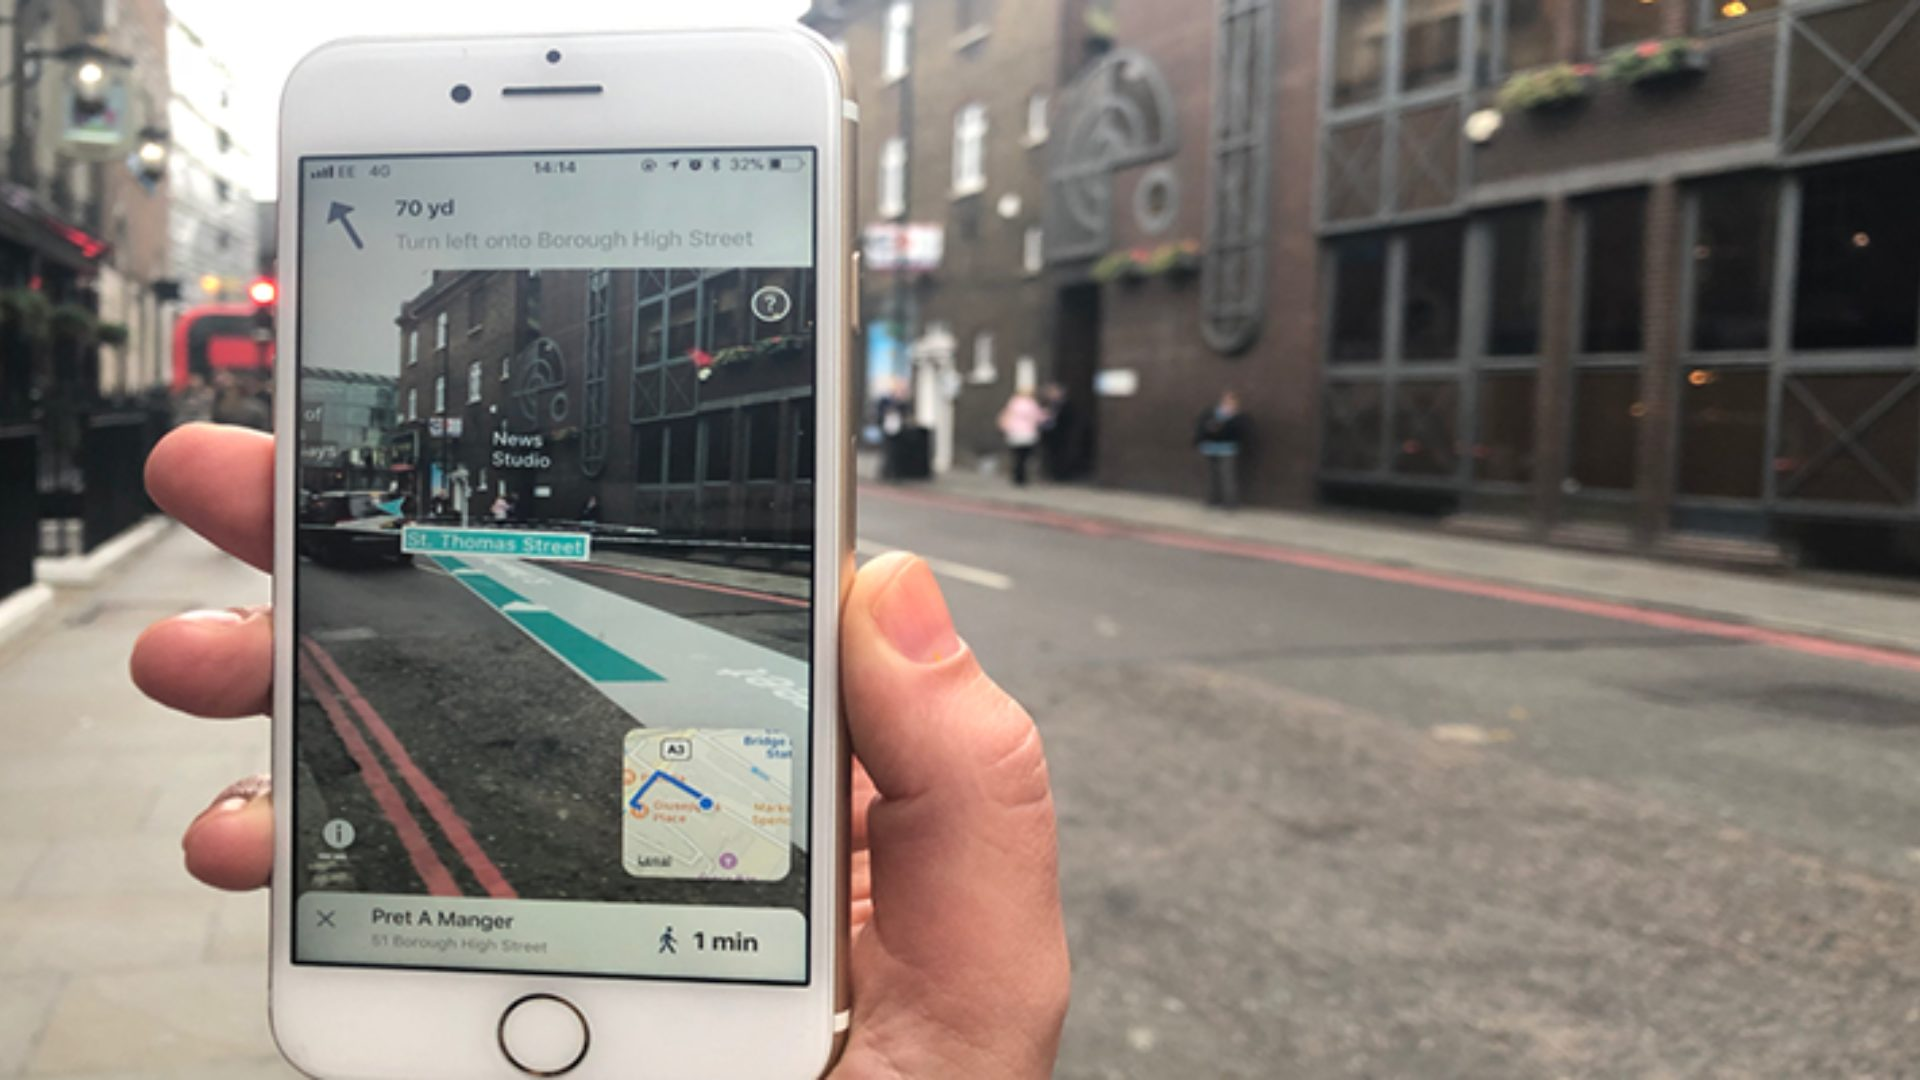
\includegraphics[width=\columnwidth, clip]{arcity.jpg}}
      \caption{(脚注\ref{footnote:arcity}より図引用)}
      \label{figure:koch}
    \end{figure}

    Vision--based ARはさらにマーカ有りとマーカレスに分類できる.
    マーカを用いた屋内ナビゲーションシステムの例として,吉野らは,迷いやすい人の特徴を考慮した上で,QRコードマーカを目印とし,スマートフォン画面上にARで進むべき方向の矢印を表示する屋内ナビゲーションシステム``DoCoKa''を開発している\cite{Yoshino:2013}.
    Kochらは,出口の案内板など自然なオブジェクトをARマーカとしたナビゲーションシステムを開発している\cite{Koch:2014}.これにより,屋内において煙が探知された際に,作動した煙探知機までの経路を提示し,ARを用いて対処方法を提示している.
    \begin{figure}[tb]
      \centerline{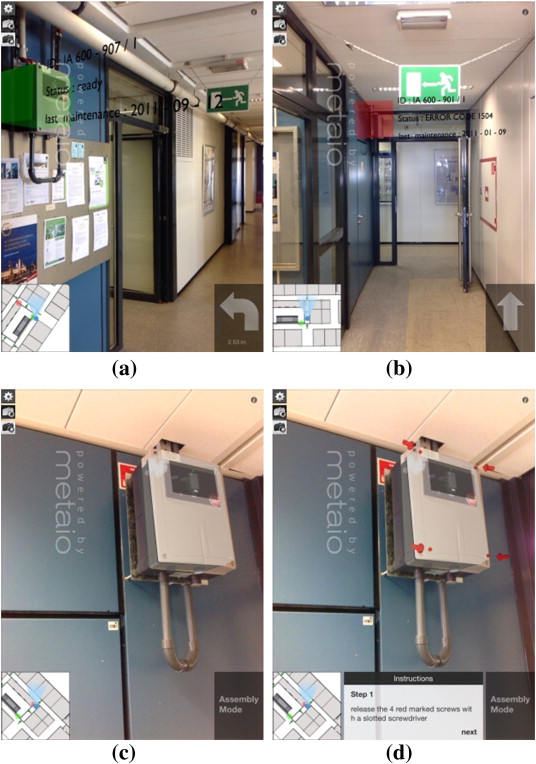
\includegraphics[width=\columnwidth, clip]{koch.png}}
      \caption{(文献\cite{Koch:2014}より図引用)}
      \label{figure:koch}
    \end{figure}

    マーカレスARを用いた屋内ナビゲーションシステムの例として,
    Georgらは,屋内など限定された地域におけるナビゲーションシステムを提案している\cite{Gerstweiler:2018, Iwanaji:2016}.
    しかし,これらのVision--based ARのみを用いたシステムは,屋内など特定の場所でしか利用できない.
    
    このような携帯端末上でのARを用いたナビゲーションは,紙の地図を用いた場合と比較して,より短い時間と少ない操作で目的地まで辿り着けることが明らかとなっている\cite{Rehman:2017, Yoshino:2013}.
    

\section{情報の視認性に関する研究}
  畑らは,画像内に高解像度領域と低解像度領域を作ることによって,ユーザに気づかせることなく視線を特定の領域に誘導させる手法を提案している\cite{Hata:2016}.
  例として,図\ref{figure:hata} --(a)に示す画像をユーザに提示すると,ユーザの視線がどこに集中しているかを示すヒートマップは図\ref{figure:hata} --(b)のようになる.
  \begin{figure}[tb]
    \begin{minipage}{0.49\hsize}
      \begin{center}
        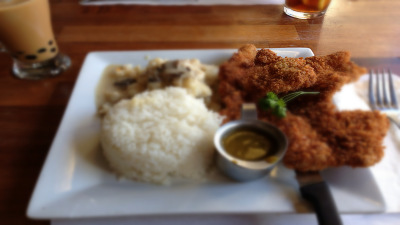
\includegraphics[clip, width=\textwidth]{hata1.png}\\
        \small{(a)提示画像}
      \end{center}
    \end{minipage}
    \begin{minipage}{0.49\hsize}
      \begin{center}
        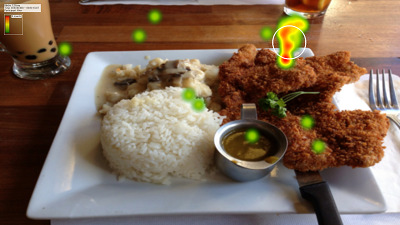
\includegraphics[clip, width=\textwidth]{hata2.png}\\
        \small{(b)ヒートマップ}
      \end{center}
    \end{minipage}
    \vspace{2pt}
    \caption{解像度制御による視線誘導(文献\cite{Hata:2016}より図引用)}
    \label{figure:hata}
  \end{figure}

  拡張現実感とは対称に,隠消現実感(Diminished Reality; DR)の研究が行われている\cite{Mori:2017}.
  DRとは,実世界から図\ref{figure:mori} --(a)のように色情報を取り除いたり,図\ref{figure:mori} --(b)のように物体を透視したり,図\ref{figure:mori} --(c)のように特定の物体を置き換えたり,図\ref{figure:mori} --(d)のように特定の物体を消去したりする技術の総称である.
  \begin{figure}[tb]
    \centerline{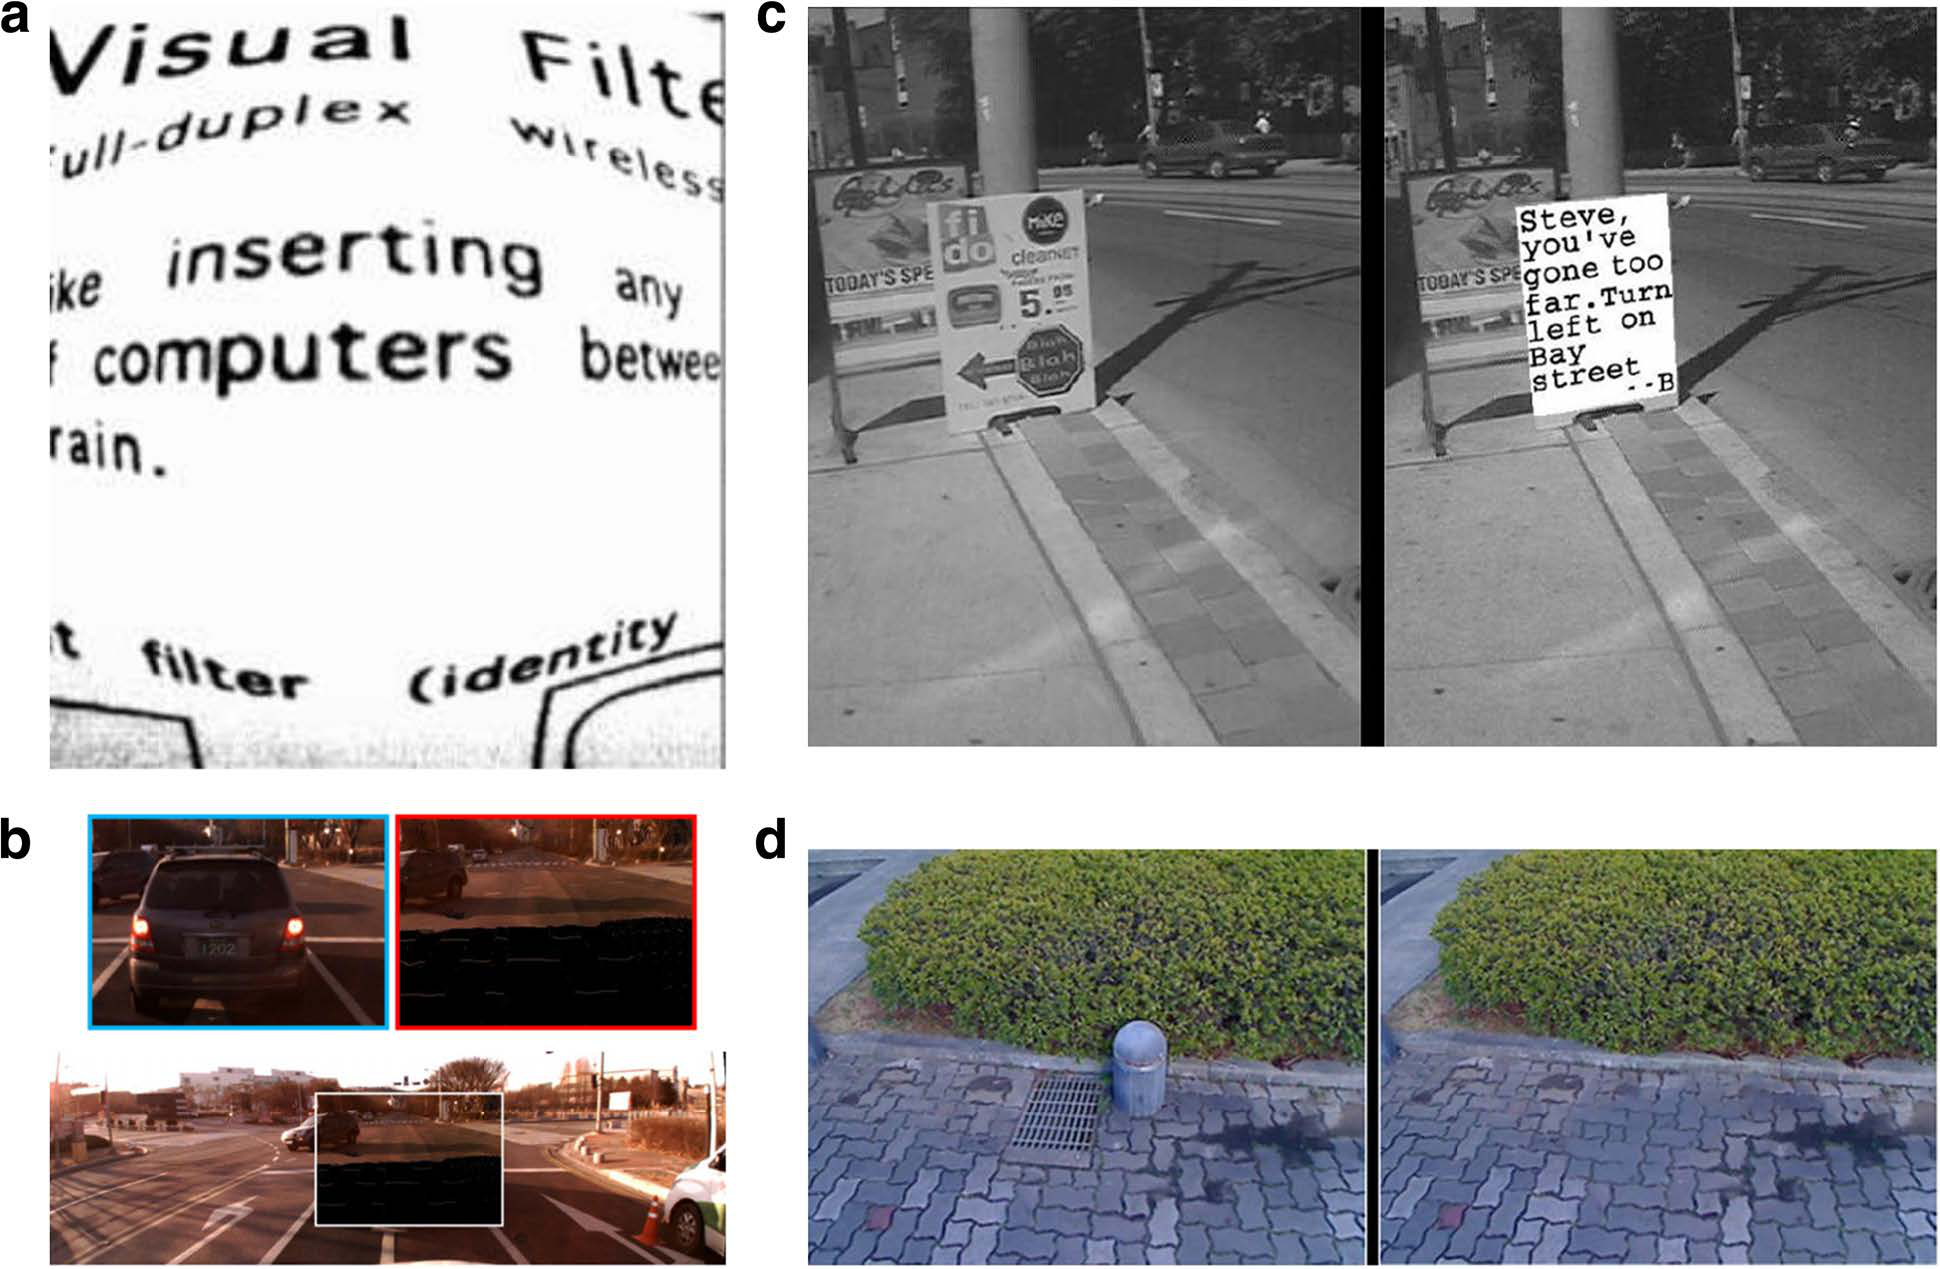
\includegraphics[width=\columnwidth, clip]{mori.png}}
    \caption{隠消現実感(文献\cite{Mori:2017}より図引用)}
    \label{figure:mori}
  \end{figure}

\section{看板認識に関する研究}
  看板に書かれてある文字を認識する研究は多数行われている.
  主な手法としては,ニューラルネットワークを用いて看板に書かれている文字を認識する手法や,Optical Character Recognition(OCR)を用いる手法が挙げられる.
  Heらは,シーケンスラベリング問題として背景から文字を読み取る再帰型ニューラルネットワークを開発している\cite{He:2016}.
  Leeらは,特徴量を用いてストリートビュー画像から文字領域を検出する手法を提案し,OCRソフトウェアが文字認識することを容易にしている\cite{Lee:2016}.
  しかし,看板の中には手書き文字など崩した文字で書かれているものもあり,人間であっても読むことが容易でない場合がある.このような場合は,OCRを用いて文字を認識することは困難である.
  Kavatiらは,図\ref{figure:kavati}のようにスマートフォンで撮影された看板や標識の写真内の文字をOCRによって認識し,英語からテルグ語に翻訳してユーザに提示する旅行者向けのWebアプリケーションを開発している\cite{Kavati:2017}.
  \begin{figure}[tb]
    \begin{minipage}{0.49\hsize}
      \begin{center}
        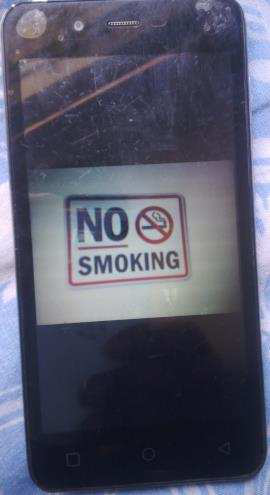
\includegraphics[clip, width=\textwidth]{kavati1.png}\\
        \small{(a)英語}
      \end{center}
    \end{minipage}
    \begin{minipage}{0.49\hsize}
      \begin{center}
        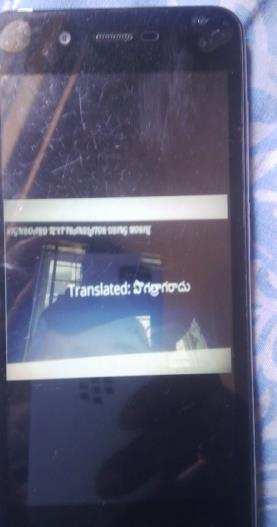
\includegraphics[clip, width=\textwidth]{kavati2.png}\\
        \small{(b)テルグ語}
      \end{center}
    \end{minipage}
    \vspace{2pt}
    \caption{翻訳された看板の文字(文献\cite{Kavati:2017}より図引用)}
    \label{figure:kavati}
  \end{figure}
  
\section{物体認識に関する研究}

\section{本研究の位置付け}

\chapter{デザイン指針}
\label{chapter:design_guidline}
本章では,提案システムのデザイン指針について述べる.

\section{これまでの取り組み:減算型表示}
\label{section:dr_method}
  \ref{subsection:signboards_in_town}節で述べたように,繁華街には看板などの視覚情報が氾濫しているため,どの情報がユーザにとって必要なものかを見分けることが難しい.
  加藤らは,複数の視覚表示が同時に提示される際,表示数が多くなるほど情報を取得する時間が増加することを示している\cite{Kato:2008}.
  このため,視覚情報が溢れている環境の中においては,ユーザが同時に見る情報量を減らすことによって,求める条件に合致する店舗の探索が容易になることが期待される.
  一方,看板など店舗の外観から得られる情報量には限度があるため,ARを用いて詳細情報を重畳表示することによって,ユーザが看板から取得できる情報量が増加することが期待される.

  これまでの研究動向として,藤田らは,ARを用いて情報を重畳することで必要な情報を目立たせる手法を「加算型の情報提示」,DRのアプローチを取り入れることで不要な情報を目立たなくさせる手法を「減算型の情報提示」と位置付け,減算型情報提示手法を提案した\cite{Fujita:2013}.減算型情報提示手法において適切な情報削除の方法を検証するために,藤田らは以下に示す3種類の手法を用いて画像から不要な情報を減算し,情報探索の所要時間を計測する実験を行った.
  \begin{itemize}
    \item 白黒:不要な情報の彩度をなくしたもの
    \item ぼかし:不要な情報の輪郭情報をなくしたもの
    \item 白黒とぼかし:不要な情報の彩度と輪郭情報をなくしたもの
  \end{itemize}
  実験は,ユーザが街の中で減算型情報提示手法を用いたシステムを使うことを想定し,上記の手法で情報を減算した画像を携帯端末に表示して行われた.実験開始前に探索する看板の店舗名のみを実験参加者に教示し,その看板を見つけるよう指示を出した.実験開始から教示した看板を発見するまでの時間を計測した.実験の結果,探索時間は削減方法の差による影響を受けないことが示唆された.また,アンケートで最も良かった減算手法について質問したところ,白黒が過半数を超えた.そこで本研究では,情報の削減手法に白黒を用いて実験を行う.藤田らの実験では,看板の多い環境において減算型情報提示手法の優位性を確認するために,既存の情報にARを用いて情報を加算する従来の手法(加算型情報提示手法)と,DRのアプローチを用いて不要な情報を減算する提案手法(減算型情報提示手法)との比較を行い,それぞれの探索時間を比較が行われた.加算型情報提示手法を適用する画像は,画像の中にある探索対象の看板に緑色の吹き出しを追加し,その中に店舗名を表示した.一方,減算型情報提示手法を適用する画像には,探索対象の看板以外の情報を白黒にした.実験から得られた探索時間の結果を比較したところ,減算型情報提示手法に優位性は見られなかった.このため,加算型情報提示手法と減算型情報提示手法には差がないことが示唆された.

  減算型情報提示手法の問題点として,不要な情報を減算する際,対象となる看板の色が白黒であり,かつその周辺の景色の彩度が低い場合がある.
  例として,新日本新地ビル\footnote{大阪府大阪市北区曾根先新地1-7-8}付近で撮影した図\ref{figure:kitashinchi}--(a)の写真から,``春雨''以外の看板情報を減算すると,図\ref{figure:kitashinchi}--(b)のようになる.
  このような場合,看板の視覚情報が減算された周囲の視覚情報と混同し,減算の効果が減少するという問題が生じる.
  この問題を解決するために,先行研究\cite{Kitamura:2017a, Kitamura:2017b}では,藤田らが提案した減算型情報提示手法を加算型で拡張し,加算型と減算型のハイブリッド型情報提示手法を提案した.

  \begin{figure}[t]
    \begin{minipage}{0.49\hsize}
        \begin{center}
          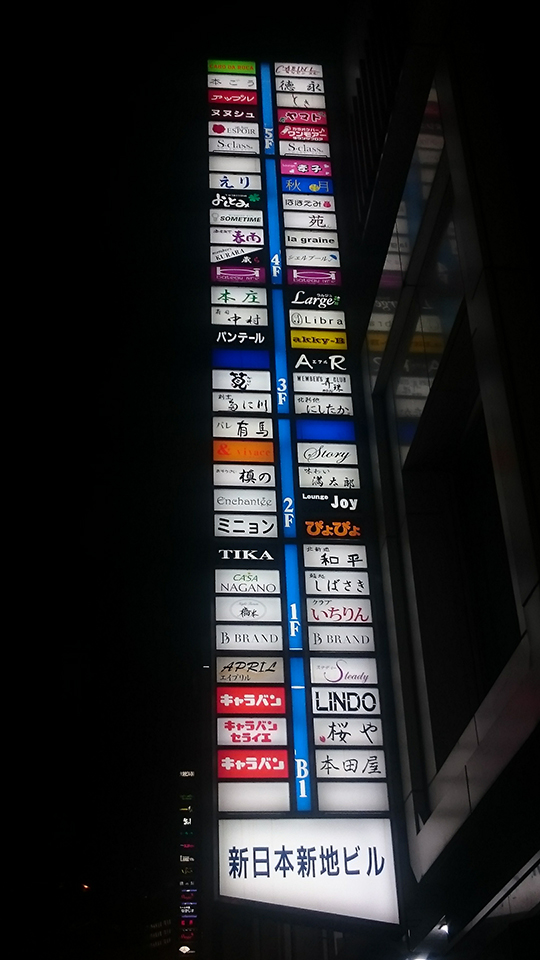
\includegraphics[clip, width=\textwidth]{kitashinchi1.png}\\
          \small{(a)加工前}
        \end{center}
    \end{minipage}
    \begin{minipage}{0.49\hsize}
        \begin{center}
          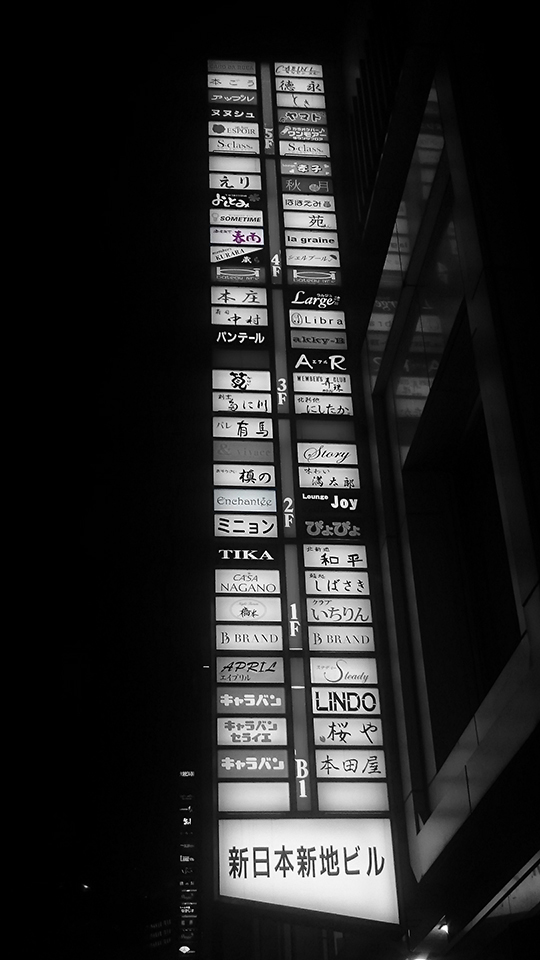
\includegraphics[clip, width=\textwidth]{kitashinchi2.png}\\
          \small{(b)加工後}
        \end{center}
    \end{minipage}
    \vspace{2pt}
    \caption{彩度が低い看板(文献\cite{Kitamura:2017a}より図引用)}
    \label{figure:kitashinchi}
  \end{figure}

  \subsection{減算型表示のインタフェース}
    減算型表示のインタフェースは,文献\cite{Fujita:2013}で提案された減算型情報提示手法をベースとする.
    しかし,不要な情報を減算するのみでは,周辺の景色の彩度が低い場合など,環境条件によっては減算の効果が得られないことがある.そこで先行研究\cite{Kitamura:2017a, Kitamura:2017b}で提案された,ARを用いて文字情報を付加したハイブリッド型情報提示手法用いたインタフェースとする.
    文字色は背景の色に合わせて変化させる.これにより,ユーザが求める情報のみが分かりやすく提示されるため,上記の問題の解決が期待される.
    提案システムでは,ユーザが目的の店舗名や店舗の種類をクエリとして入力する.
    ユーザが入力したクエリに一致する視覚情報はユーザにとって必要な情報であり,それ以外の視覚情報は不要な情報である.
    そのため,情報の識別性向上を目的として,図\ref{figure:dr_method}に示すような出力をユーザに提示する.
    これは,不要な視覚情報をグレースケール化することによって減算し,必要な視覚情報には店舗名などの文字情報を看板の横に重畳して表示したものである.
    これにより,ユーザは不要な視覚情報を完全に失うことなく,必要な視覚情報のみを得られることが期待される.

    \begin{figure}[tb]
      \centerline{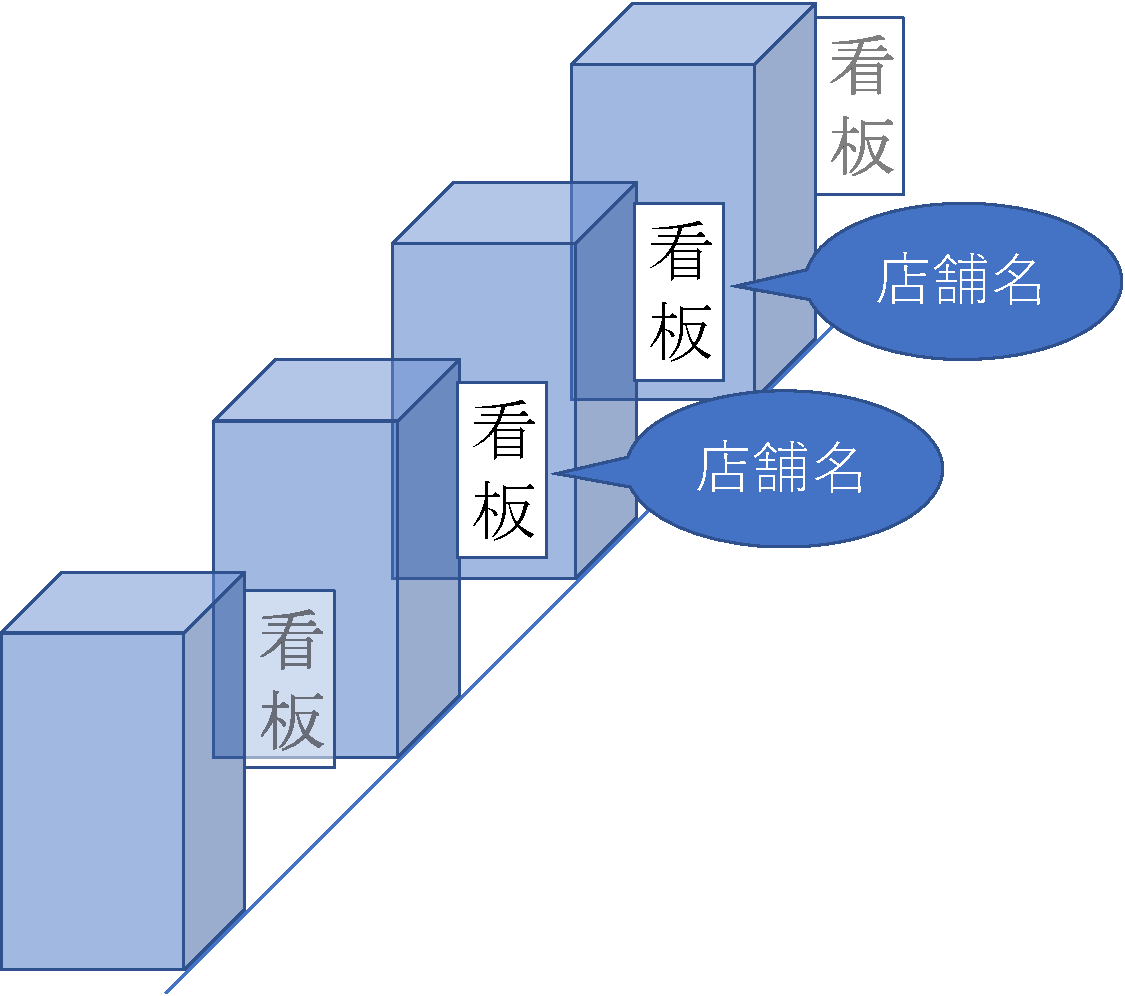
\includegraphics[width=\columnwidth, clip]{dr_method.pdf}}
      \caption{減算型表示の出力イメージ(文献\cite{Kitamura:2017a}より図引用)}
      \label{figure:dr_method}
    \end{figure}

\section{対象とする状況}
\label{section:target_situation}
  本研究では,\ref{section:purpose}節で述べた目的を実現するために,都市部や繁華街などの店舗が多数存在している地域において,観光客などその地域に慣れていないユーザが携帯端末を手に持って情報を探索する状況を対象とする.本稿で対象とする状況は以下の2つである.
  \begin{enumerate}
    \item 看板などの周囲の視覚情報が多すぎるため,目的地の看板は目に入っているものの,周辺の過剰な視覚情報に埋没して,素早く見つけることが困難である状況,
    \item 目の前にある店舗の情報が知りたいが,その地域に慣れていないことや言語障壁などの問題によって,その店舗の詳細情報を知ることが困難である状況,
  \end{enumerate}
  (1)に対しては,過剰に存在する視覚情報の中から,ユーザにとって不要な情報を低減することによって,情報の視認性の向上を実現する.この手法を``減算型表示''と定義し,視覚情報が密集している地域においてユーザが必要とする情報を素早く発見できるシステムを実装する.
  (2)に対しては,看板画像を認識し,オープンデータを用いて看板から店舗情報を取得することによって,目の前にある店舗の詳細情報を直感的かつ容易に得られるようにする.この手法を``Search by Snap''と定義し,ユーザが店舗の看板にモバイルデバイスのカメラを向けるだけでその店舗の情報が得られるシステムを実装する.
  
\section{提案システムの要件}
  \label{subsection:requirement}
  \ref{section:target_situation}節で述べた問題を解決し,素早く目的の情報にアクセスするために必要な要件として,以下の4点を定義する.
  \begin{enumerate}
    \item ユーザが求める店舗情報の探索が直感的にできる操作方法であること
    \item ユーザがカメラを通して見た店舗の看板と端末の画面上に表示される付加情報とのシームレスな連携が可能であること
    \item 周囲に店舗が密集している場合においても,ユーザが必要とする看板情報を迷わずに探索できること
    \item 天候や時間帯などの環境条件に左右されず,ユーザに迷わせることなく情報の提示ができること
  \end{enumerate}
  本稿で提案するシステムは,モバイルデバイス上で実行することを想定している.システムを実現するにあたり,上述した(1)と(2)を満たすために,
  \begin{itemize}
    \item ユーザが店舗名や店舗の種類をクエリとして検索するために,システムを利用する地域における店舗の種類,名称及びその看板画像の組がデータベースとして用意されていること
    \item リアルタイムで看板認識を行うために,モバイルデバイスは動画の撮影が可能であり,端末上またはサーバ上でリアルタイムで画像処理が行える環境が存在すること
    \item サーバ上にあるデータベースにアクセスするために,Long Term Evolution(LTE)やWi-Fiなどの方法でインターネットにアクセスできること
    \item 歩きながら端末を操作することは危険であり,ユーザは立ち止まって片方の手でモバイルデバイスを持ち,もう片方の手でシステム操作を行うことが望ましいため,片手で操作できるサイズの端末であること
  \end{itemize}
  の4点を前提条件として想定する.

\section{提案手法:Search by Snap}
\label{section:design_sbs}
  \ref{section:searching_action}節で述べたように,ユーザが慣れていない地域や言語障壁のある地域において,目の前にある店舗で受けられるサービスの詳細やクレジットカードでの支払いの可否や,店内での喫煙の可否等の詳細情報を瞬時に把握することは困難である.
  これらの情報は,店舗のWebサイトや飲食店の情報が掲載されているWebサービス等から取得する必要がある.
  この問題を解決するために,ユーザが携帯端末に搭載されているカメラを通して目の前の店舗の看板を見ることで,求める情報に効率良くアクセスできるようにする.
  
  \subsection{提案インタフェースのデザイン}
    \ref{subsection:requirement}節で述べた(3)を満たすために,飲食店における予算や提供されている料理の種類,クレジットカードでの決済の可否など,ユーザが求めている条件をクエリとして入力でき,減算型表示のアプローチを用いてユーザにとって不要な情報は目立たなく表示するインタフェースとする.
    \ref{subsection:requirement}節の(4)を満たすために,減算型表示と同様に,条件に合致しない看板情報の色調を低減させ,条件に合う看板のみを強調して表示するインタフェースとする.
    提案インタフェースの出力イメージを図\ref{figure:sbs_method}に示す.
  \begin{figure}[tb]
    \centerline{
\includegraphics[width=\columnwidth, clip]{sbs_method.pdf}}
    \caption{Search by Snapの出力イメージ}
    \label{figure:sbs_method}
  \end{figure}

\chapter{実装}
\label{chapter:proposal}

\section{減算型表示のプロトタイプ}
  \begin{figure}[t]
    \begin{center}
    \begin{minipage}{0.3\hsize}
        \begin{center}
            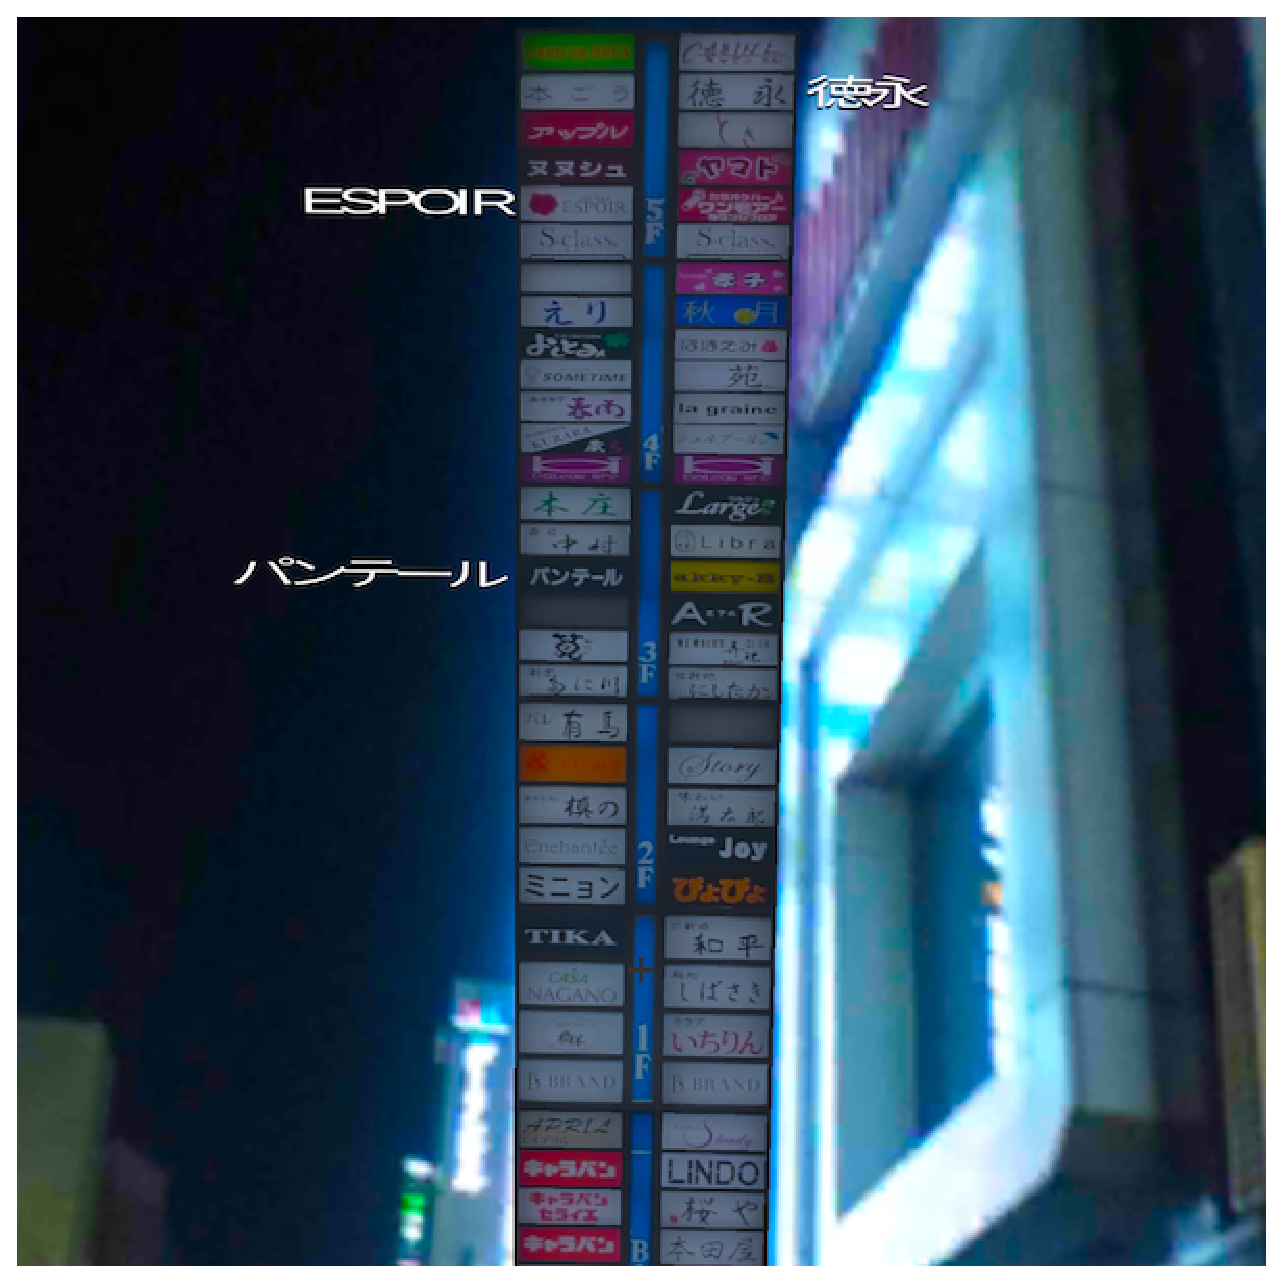
\includegraphics[clip, width=.95\textwidth]{dr_method1.eps}\\
            \small{(a) 加算型}
        \end{center}
    \end{minipage}
    \begin{minipage}{0.3\hsize}
        \begin{center}
            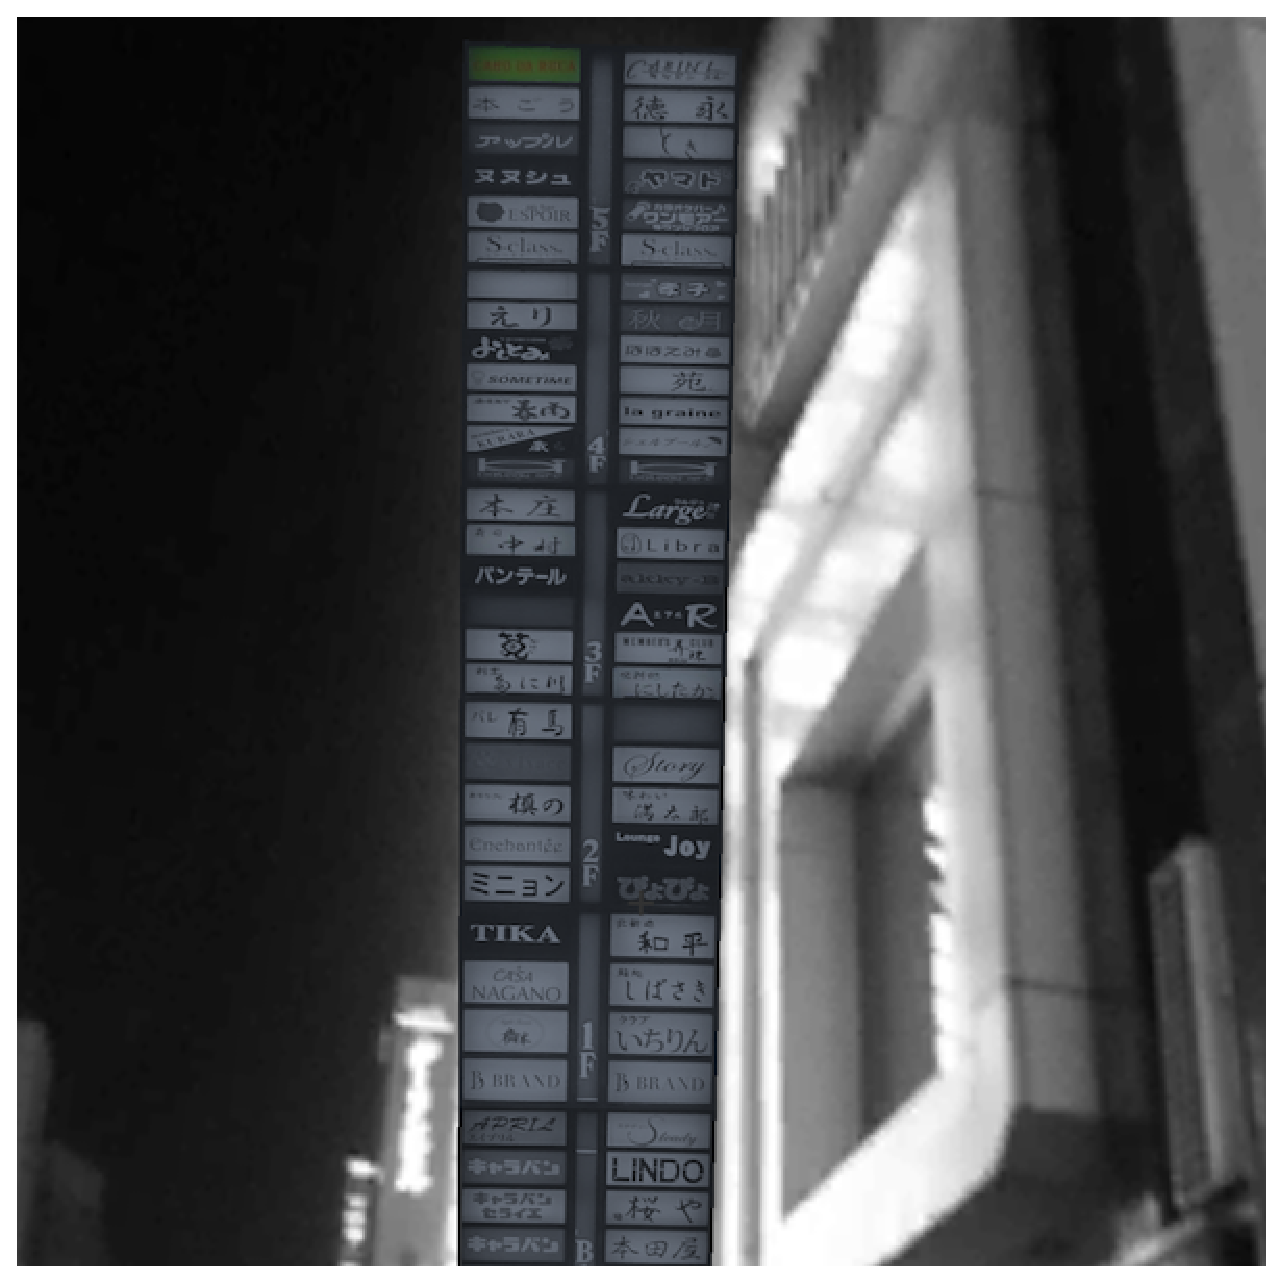
\includegraphics[clip, width=.95\textwidth]{dr_method2.eps}\\
            \small{(b) 減算型}
        \end{center}
    \end{minipage}
    \begin{minipage}{0.3\hsize}
        \begin{center}
            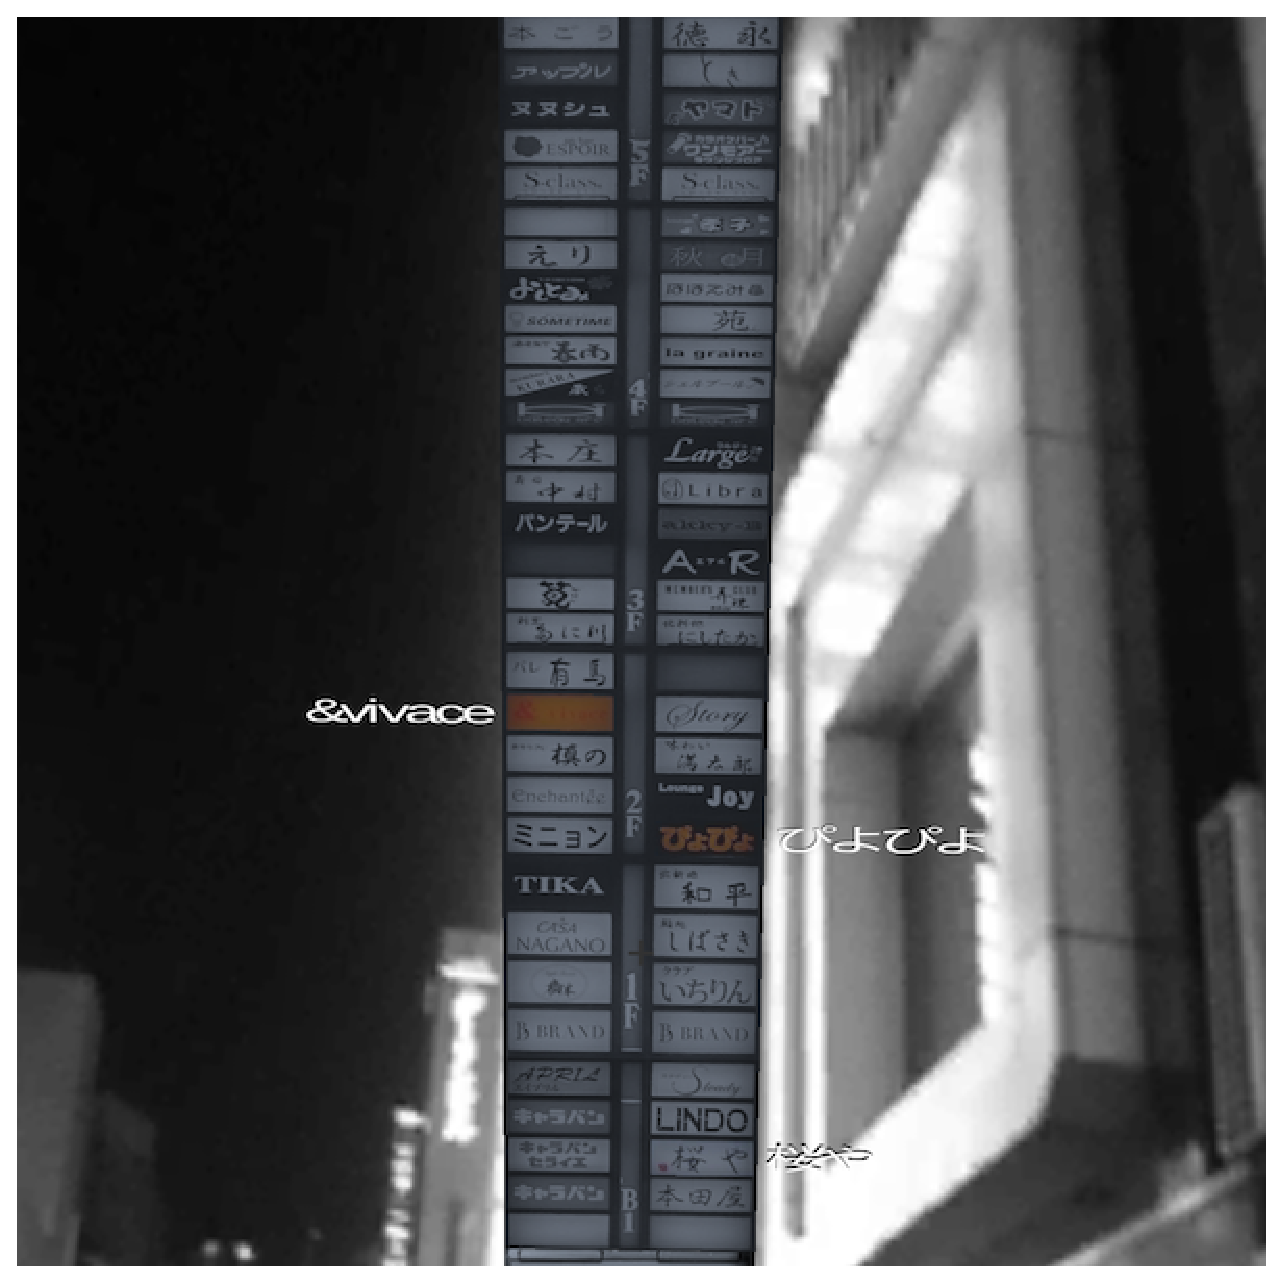
\includegraphics[clip, width=.95\textwidth]{dr_method3.eps}\\
            \small{(c) ハイブリッド型}
        \end{center}
    \end{minipage}
    \end{center}
    \vspace{1pt}
    \caption{プロトタイプの出力画面}
    \label{fig:prototype}
  \end{figure}
  本節では,?章で述べる実験に用いるプロトタイプシステムについて述べる.実験用のプロトタイプは,モバイルデバイス上で実行できるようUnity(ver 5.6.0f3)を用いてC\#言語で実装した.実環境に近づけるために,RECOH THETA\footnote{\url{https://theta360.com/}(2017/4/27確認)}を用いて新日本新地ビル付近で撮影した昼と夜の全天球画像を用意し,モバイルデバイスを通して見回せるようにした.全天球画像では看板が鮮明に撮影できないため,看板は別に撮影した画像をオブジェクトとして設置した.

  実験に用いる看板情報は,図\ref{fig:kitashinchi} - (a) に示す大阪府北新地の新日本新地ビルに掲示されている61枚の看板を用いた.店舗の種類は北新地総合情報サイト\footnote{\url{http://kgnet.jp/}(2017/4/27確認)}を参考に,「スナック・ラウンジ」,「バー」,「和食」,「居酒屋」,「クラブ」,「寿司」,「中華料理」,「ドレスショップ」の8種類に分類した.サイトに記載がなかった店舗は,「その他」として分類した.データベースはSQLite\footnote{\url{https://www.sqlite.org/}(2017/4/27確認)}(ver 3.8.10.2)を用いて,画像内の看板の位置,店舗の名前,店舗の種類,看板画像をそれぞれ格納した.

  プロトタイプでは,ユーザはモバイルデバイスを全天球画像内で全方向に向けることができる.画面中央に照準を表示し,システムは照準のローカル座標と看板のワールド座標を対応させることにより,特定の看板が選択されたことを認識できる.情報提示手法に関しては,
  \begin{itemize}
    \item 加工なし(以下,通常型と記す)
    \item 看板の横に店舗名を表示(図\ref{fig:prototype} - (a) ,以下,加算型と記す)
    \item 特定の看板以外の情報をグレースケール化(図\ref{fig:prototype} - (b) ,以下,減算型と記す)
    \item 特定の看板以外の情報をグレースケール化し,看板の横に店舗名を表示(図\ref{fig:prototype} - (c) ,以下,ハイブリッド型と記す)
  \end{itemize}
  の4種類を切り替えられるようにし,探索対象の看板は,店舗の種類別に切り替えられるようにした.また,ユーザがスタートボタンをタップしてから特定の看板を見つけるまでの所要時間を計測できる機能を用意した.ユーザが特定の看板に照準を1秒間合わせると,看板を見つけたと判定するよう実装した.

\section{リアルタイム看板認識APIの実装}

    \begin{table}[t]
    \caption{プロトタイプに用いたデータ(2018年12月時点OSMのデータベースを基に作成)}
    \label{tab:storelist}
    \begin{center}
      \begin{small}
        \begin{tabular}{c|cccccc}
        \hline\hline
        id & name & shop/amenity & opening\_hours & payment:visa \\ 
        \hline
        2391866925 & セブン-イレブン 高槻高槻町店 & convenience & 24/7 & yes \\
        5279265335 & 全席個室居酒屋 北海の恩返し 高槻店 & bar & 17:00-24:00 & yes \\
        5281672553 & 小だるま JR高槻駅前店 & bar & Mo-Th 11:30-14:00; \ldots & yes \\
        5281672555 & 肉丼専門店 高槻肉劇場 & restaurant & 11:00-23:00 & no \\
        5281672556 & おだいどこはなれ 高槻店 & bar & Mo-Th 11:30-24:00; \ldots & yes \\
        5281672557 & ビリヤード・ダーツ\&Food Bar Ozbuddy & pub & Mo-Th 14:00-26:00; \ldots & no \\
        5281672577 & 磯丸水産 高槻店 & restaurant & 24/7 & yes \\
        5281672578 & 炭焼酒場 森田家 高槻店 & restaurant & 17:00-26:00 & yes \\
        5281672579 & メサベルテ 高槻店 & bakery & Mo-Sa 07:00-20:30; \ldots & no \\
        5281672580 & 駿河屋 & hobby & 10:00-23:00 & no \\
        5281672581 & 甲南チケット 高槻本通店 & ticket & Mo-Sa 10:00-19:00; \ldots & no \\
        5281672739 & 焼肉・しゃぶしゃぶ食べ放題ぷくぷく 高槻店 & restaurant & Mo-Fr 16:30-25:00; \ldots & yes \\
        5281672740 & 赤から 高槻店 & bar & Mo-Fr 17:00-24:00; \ldots & yes \\
        5281672835 & ちどり亭 高槻店 & restaurant & 17:00-25:00 & yes \\
        5281672942 & 高槻ちゃぶちゃぶ & bar & 17:54-06:00 & yes \\
        \hline
        \end{tabular}
      \end{small}
    \end{center}
    \end{table}

    \begin{table}[tb]
        \caption{看板画像の学習と検出に用いたマシンのスペック}
        \label{tab:machine}
        \begin{center}
        \begin{tabular}{c|c}
            \hline\hline
            要素 & スペック \\
            \hline
            CPU & Intel (R) Core (TM) i7-8700K @ 3.70 GHz \\
            RAM & 16 GB \\
            GPU & NVIDIA GeForce GTX 1080 \\
            VRAM & 12 GB \\
            OS & Ubuntu 17.10 \\
            \hline
        \end{tabular}
        \end{center}
    \end{table}

    \subsection{対象とするデータ}
    \ref{sec:system}章で述べた構成に基づき,大阪府高槻市のJR高槻駅と阪急高槻市駅の間にある商店街の一部を対象としたプロトタイプを実装する.看板の認識には,少ない学習データから高い精度での認識を可能にするために,文献\cite{Kitamura2018}で提案したAPIを用いる.
    プロトタイプでは,図\ref{fig:map}の赤線部で示されている高槻本通の$100 m$区間においてOSM上にデータが存在する店舗のうち,15店舗を対象とする.
    対象とする店舗のノードを表\ref{tab:storelist}に示す.
    OSM上では,飲食店などの店舗のオブジェクトは位置を定義された単一の点であるノードとして扱われ,各オブジェクトには``OSM ID''という一意の番号が付与されている.
    各店舗の看板画像とOSM IDを紐付け,Overpass API\footnote{http://overpass-api.de}を用いて店舗情報を取得することにより,看板画像から店舗情報へのアクセスができる.
    表\ref{tab:storelist}内の``id''は各店舗のOSM IDを表しており,それぞれのノードには複数のタグが設定されている.
    ``name''は店舗の名称が代入されている.
    ``shop''タグは,店舗が販売している商品を記述するために使用される.
    飲食店の場合,施設の種類を表す``amenity''タグにバーやレストランのような店舗の種類が代入されている.
    ``opening\_hours''タグには,店舗の営業時間が代入されている.年中無休で24時間営業の場合は``24/7''が,曜日によって営業時間が異なる場合は,セミコロン区切りで複数の値が代入されている.例えば,小だるま JR高槻駅前店は,月曜日から木曜日までは11時30分から14時00分と17時から23時30分まで,金曜日,土曜日は11時30分から14時30分と17時00分から24時30分,日曜日は11時30分から23時30分が営業時間である.この場合,``opening\_hours''タグの値は
    ``Mo-Th 11:30--14:00, 17:00--23:30; Fr-Su 11:30--14:30, 17:00--24:30; Su 11:30--23:30''となる.
    支払いにクレジットカードが利用可能かどうかは,``american\_express'',``payment:diners\_club'',``payment:jcb'',``payment:master'',``payment:visa'',のタグに``yes''が代入されていれば利用可能である.表\ref{tab:storelist}には``payment:visa''タグのみを掲載している.

  \subsection{看板画像の学習}
    看板の認識は,まず写真の中から看板領域を抽出し,次に,切り出された看板がどの店舗のものなのかを識別するという2段階で行う.
    看板画像の学習は,文献\cite{Kitamura2018}と同一の条件下で行った.学習に用いたマシンのスペックを表\ref{tab:machine}に示す.
    写真の中から看板の領域を抽出するために,Tensorflow 1.0\cite{abadi2016tensorflow}で実装されたYOLOv2\cite{YOLO9000}を用いた.
    対象とする店舗の前で様々な角度から合計650枚の写真を撮影し,それぞれに人手で看板領域をアノテーションした上で,585枚を教師データ,65枚をテストデータとして学習させた.

    抽出した看板画像から店舗名を識別するためには,VGG16\cite{VGG16}を用いた.
    表\ref{tab:storelist}に記載した15店舗の看板画像を昼の時間帯に各店舗100枚ずつ,合計1,500枚の写真を収集し,1店舗につき教師データ50枚,バリデーションデータ25枚,テストデータ25枚に分類して学習させた.

    看板認識を行うAPIは,Python \footnote{https://www.python.org} 3.6.5とWeb APIフレームワークであるFalcon \footnote{https://falconframework.org} 1.4.1を用いて,を用いて学習に用いたマシンと同一のマシンに構築したサーバ上に構築した.

\section{Scan by Snapのプロトタイプ}

\begin{figure*}[t]
    \begin{center}
      \includegraphics[clip, width=1.9\columnwidth]{recog_method.eps}
      \caption{システムの動作}
      \label{fig:method}
    \end{center}
  \end{figure*}

\subsection{ユーザインタフェース}
クライアントサイドは,ユーザがOSを問わずに携帯端末で実行できるようにするために,HTML5とJavascriptを用いてWebアプリケーションとして実装した.
インタフェースはデフォルトで端末の背面カメラ画面となっており,ユーザが前面カメラと切り替えられるようになっている.
ユーザがカメラを通して店舗の看板を見ると,その店舗の店舗名,営業時間,使えるクレジットカードの種類などの情報が表示される.
表示される店舗の種類や表示する情報の種類はユーザが選択できる.
ユーザにとって不要な情報は明度を下げることによって目立たなくしている.
実装したユーザインタフェースを図\ref{fig:interface}に示す.

\subsection{システムの動作}
提案システムにおいて,ユーザが取る行動とシステムが行う処理を以下に示し,図で表したものを図\ref{fig:method}に示す.
\begin{enumerate}
    \item システムは携帯端末のGPS機能により,ユーザの位置情報を取得する
    \item ユーザは店舗の種類などのクエリを入力する
    \item システムはOverpass APIに位置情報とクエリを送信し,クエリに一致する周辺の店舗のOSM IDを取得する
    \item ユーザは携帯端末のカメラを通して街から画像情報を取得する(図\ref{fig:method}中\textcircled{\scriptsize 1})
    \item システムは画像をサーバに送信する(図\ref{fig:method}中\textcircled{\scriptsize 2})
    \item サーバはYOLOを用いて画像の中から看板領域を検出する(図\ref{fig:method}中\textcircled{\scriptsize 3})
    \item サーバは検出された看板領域を切り抜く(図\ref{fig:method}中\textcircled{\scriptsize 4})
    \item サーバはそれぞれの看板画像をVGG16を用いて店舗名でクラス分けする(図\ref{fig:method}中\textcircled{\scriptsize 5})
    \item サーバは画像内の看板の左上と右下の座標と検出した看板の店舗と関連付けられたOSMのノードのidをそれぞれ格納したJSONデータを生成する(図\ref{fig:method}中\textcircled{\scriptsize 6})
    \item サーバは生成されたJSONをシステムに返り値として返却する(図\ref{fig:method}中\textcircled{\scriptsize 7})
    \item システムはユーザが求めていない視覚情報の色調を低減させ,ユーザが求めている店舗の情報を看板の横に吹き出しとして重畳表示する(図\ref{fig:method}中\textcircled{\scriptsize 8})
    \item システムは認識した看板と関連付けられているOSM IDをOverpass APIに送信する(図\ref{fig:method}中\textcircled{\scriptsize 9})
    \item Overpass APIはOSM IDと一致する店舗のノードをシステムに返却する(図\ref{fig:method}中\textcircled{\scriptsize 10})
    \item システムは出力結果をユーザに提示する(図\ref{fig:method}中\textcircled{\scriptsize 11})
\end{enumerate}

デバイスが画像をAPIに送信してからサーバがJSONデータを返却するまでに要した時間は,上り1Mbps,下り1.25Mbpsの通信速度,980 $\times$ 1307の解像度で平均359msであった.
Thropeらによると,人間が画面中央のオブジェクトを認識するまでのリアクションタイムの中央値は445msであるため\cite{Thorpe:1996},十分にユーザが満足できる速度であるといえる.



\section{評価すべき項目の検討}
\chapter{減算型表示を用いた評価実験}
\label{chapter:experiment_dr}
本章では,減算型表示を用いて実施した評価実験と,その結果について述べる.
\section{実験の目的}
  看板密集地域において特定の看板を探索する際,加算型の情報提示手法と減算型の情報提示手法を用いたそれぞれの探索時間は,\ref{section:dr_method}節で述べたように差がないことが示唆されている.また,減算型情報提示手法には,看板や背景の彩度が低い場合に情報の識別性が加工前との変化が小さくなるという問題点がある.

  そこで本実験では,看板が密集している地域において,加算型情報提示手法と減算型情報提示手法を組み合わせた本稿の提案手法であるハイブリッド型情報提示手法を用いる.この提示手法による探索時間を従来の加算型情報提示手法,減算型情報提示手法と比較することにより,探索時間に関して提案手法の優位性を確認する.

\section{実験の概要}
  実験参加者は情報系の学部に通う大学生12名である.本実験で比較する提示手法は,\ref{chapter:implement_dr}節で述べた通常型,加算型,減算型,ハイブリッド型の4種類である.実験は\ref{chapter:implement_dr}節で述べたプロトタイプをASUS社\footnote{\url{https://www.asus.com/}(2017/4/27確認)}のNexus 7(2013,Android 6.0.1)にインストールして行った.

  実験参加者図は図\ref{figure:exp_dr_scenery}に示すように立った状態で端末を持ち,端末を全方向に向けることで全天球画像を見回し,提示された看板を探索する.ユーザが看板を記憶することを防止するために,必ず看板に背を向けた状態で実験を始めるよう指示を出した.実験の条件は,表\ref{table:exp_dr_order}に示す8通りとした.ここで探索対象の看板数に関して,単体である場合と複数である場合の2通りに区別した.これは探索対象の看板が複数である場合,不要な情報を減算する方が情報を加算することに比べてより容易に情報を探索でき,探索時間が短くなると仮説を立てたためである.

\section{実験の手順}
  初めに,端末の画面が図\ref{figure:exp_dr_procedure} - (a) の状態で実験参加者に端末を渡す.画面には探索対象の看板画像が表示されている.ユーザが開始ボタンをタップすると,図\ref{figure:exp_dr_procedure} - (b) に示す探索画面に遷移する.次に,ユーザが振り返ると,図\ref{figure:exp_dr_procedure} - (c) に示す新日本新地ビルの看板があり,ユーザはその中から探索対象の看板を探す.ユーザが探索対象の看板に1秒間照準を合わせると,図\ref{figure:exp_dr_procedure} - (d) に示す終了画面に遷移する.探索対象が複数である場合は,全ての看板を見つけた後に遷移する.

  実験では,全ての実験参加者に表\ref{table:exp_dr_order}の条件で探索してもらった.探索対象が単体である条件(表\ref{table:exp_dr_order},1〜4),探索対象が複数である条件(表\ref{table:exp_dr_order},5〜8)の順に,昼間の画像と夜の画像でそれぞれ探索してもらった.

  \begin{table}[tb]
    \caption{実験の条件}
    \label{table:exp_dr_order}
    \begin{center}
    \begin{tabular}{ccc}
      \hline\hline
      \textbf{番号} & \multicolumn{1}{c}{\textbf{提示手法}} & \textbf{対象} \\
      \hline
      1 & 通常型 & 単体 \\
      2 & 加算型 & 単体 \\
      3 & 減算型 & 単体 \\
      4 & ハイブリッド型 & 単体 \\
      \hline
      5 & 通常型 & 複数 \\
      6 & 加算型 & 複数 \\
      7 & 減算型 & 複数 \\
      8 & ハイブリッド型 & 複数 \\
      \hline
    \end{tabular}
  \end{center}
  \end{table}

  \begin{figure}[tb]
    \centerline{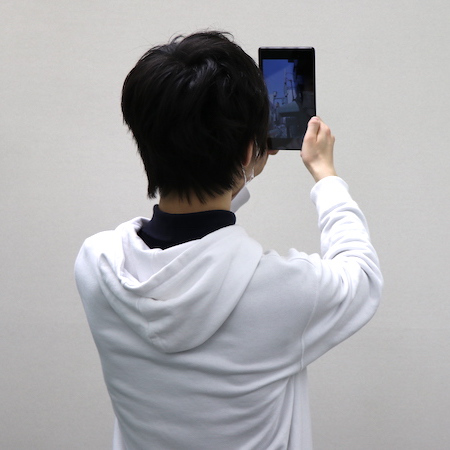
\includegraphics[width=\columnwidth, clip]{dr_exp.png}}
    \caption{実験風景(文献\cite{Kitamura:2017a}より図引用)}
    \label{figure:exp_dr_scenery}
  \end{figure}

  \begin{figure}[t]
    \begin{center}
      \begin{tabular}{cc}
        \begin{minipage}{0.45\hsize}
          \centering
          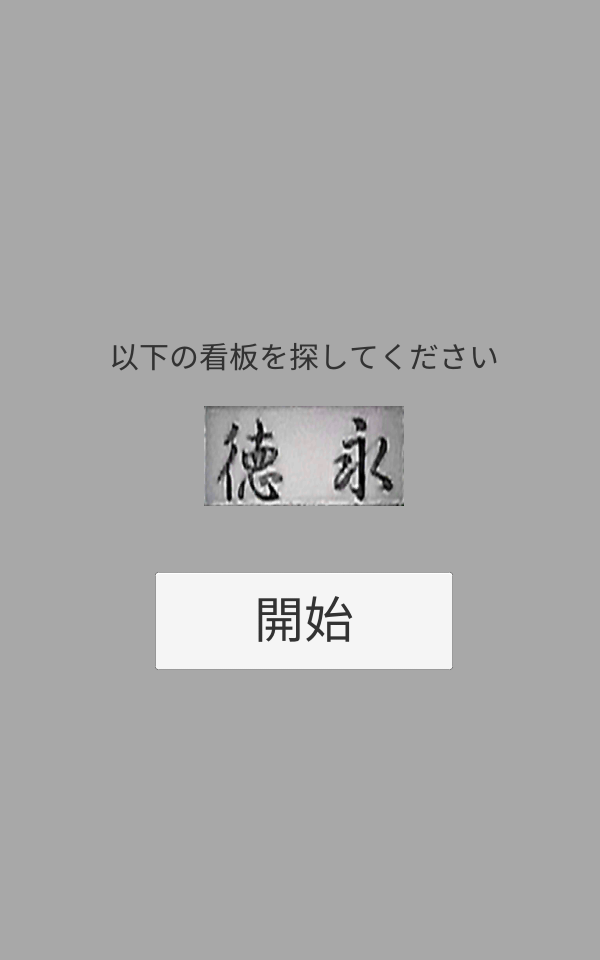
\includegraphics[clip, width=.9\textwidth]{dr_exp1.png}\\
          \small{(a)開始画面}
        \end{minipage}
        \begin{minipage}{0.45\hsize}
          \centering
          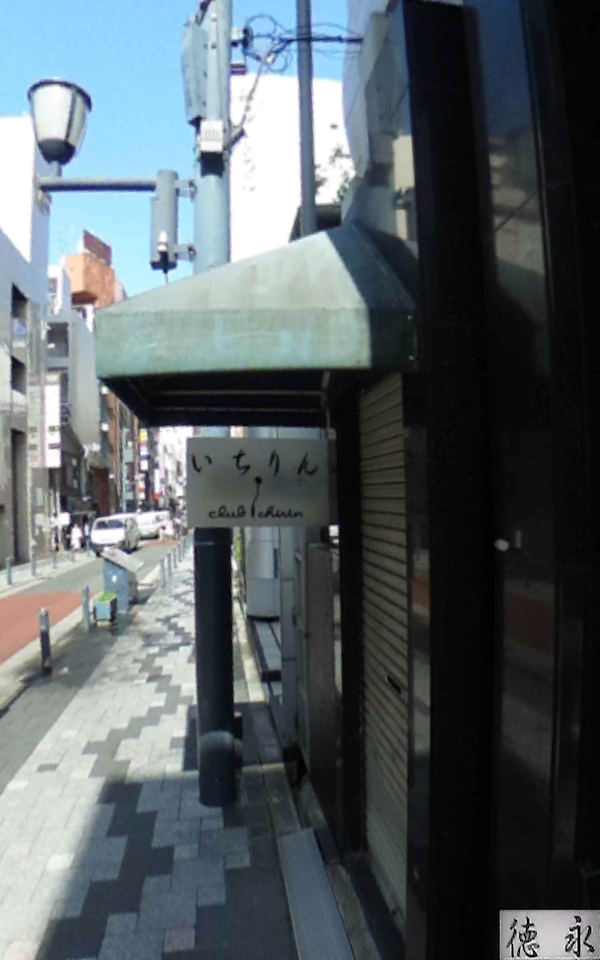
\includegraphics[clip, width=.9\textwidth]{dr_exp2.png}\\
          \small{(b)探索画面(1)}
        \end{minipage} \\\\
        \begin{minipage}{0.45\hsize}
          \centering
          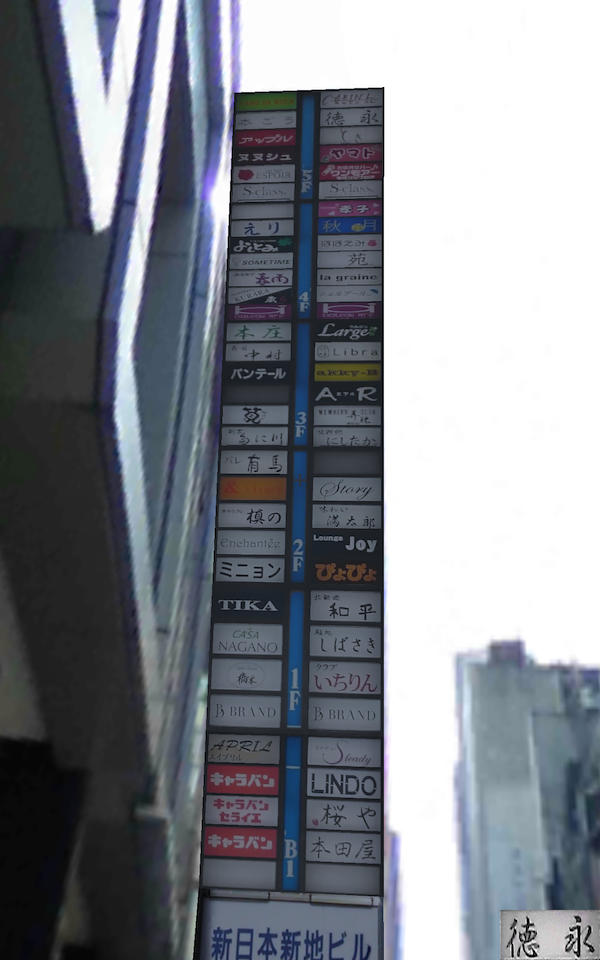
\includegraphics[clip, width=.9\textwidth]{dr_exp3.png}\\
          \small{(c)探索画面(2)}
        \end{minipage}
        \begin{minipage}{0.45\hsize}
          \centering
          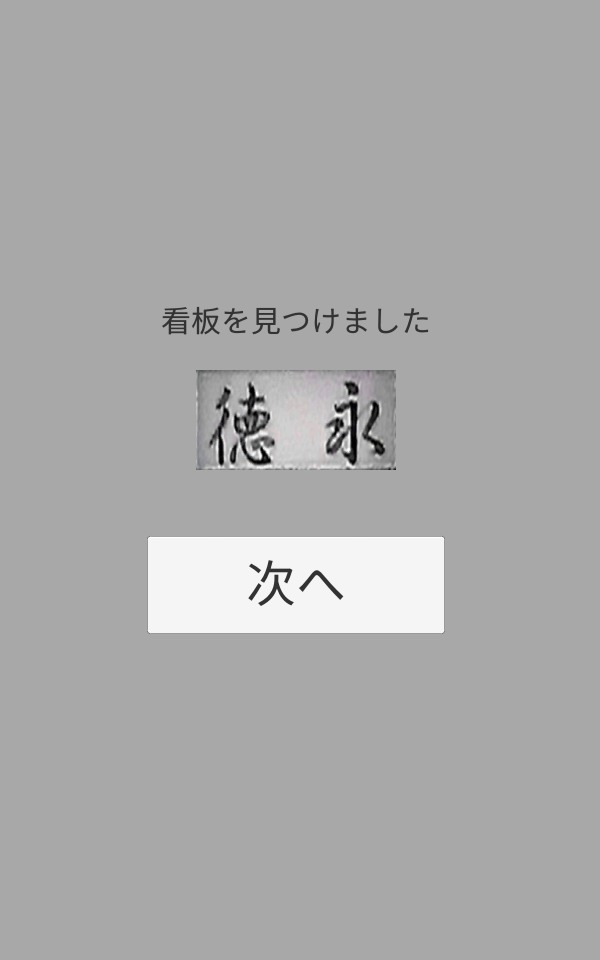
\includegraphics[clip, width=.9\textwidth]{dr_exp4.png}\\
          \small{(d)終了画面}
        \end{minipage}
      \end{tabular}
      \caption{実験の手順}
      \label{figure:exp_dr_procedure}
    \end{center}
  \end{figure}

\section{実験の結果}
  実験参加者が開始ボタンをタップしてから,指示された看板を全て見つけるまでの所要時間を計測し,通常型,加算型,減算型各々の探索時間とハイブリッド型の探索時間の平均値を比較した.その結果を以下に述べる.
  \subsection{時間帯が昼,探索対象が単体の場合}
    時間帯が昼,探索対象が単体の場合の探索時間を図\ref{figure:exp_dr_result_day} - (a) に示す.ハイブリッド型を用いた探索時間は,
    (1)通常型より有意に短い($t(22)=5.729, p<.05$)こと,
    (2)加算型より有意に短い($t(22)=2.852, p<.05$)ことが確認されたが,
    (3)減算型との間に有意差は見られなかった($t(22)=1.478, n.s.$).

  \subsection{時間帯が昼,探索対象が複数の場合}
    時間帯が昼,探索対象が複数の場合の探索時間を図\ref{figure:exp_dr_result_day} - (b) に示す.ハイブリッド型を用いた探索時間は,
    (1)通常型より有意に短い($t(22)=5.702, p<.05$)こと,
    (2)加算型より有意に短い($t(22)=6.144, p<.05$)こと,
    (3)減算型より有意に短い($t(22)=3.318, p<.05$)ことがそれぞれ確認された.

  \subsection{時間帯が夜,探索対象が単体の場合}
    時間帯が夜,探索対象が単体の場合の探索時間を図\ref{figure:exp_dr_result_night} - (a) に示す.ハイブリッド型を用いた探索時間は,
    (1)通常型より有意に短い($t(22)=4.325, p<.05$)こと,
    (2)加算型より有意に短い($t(22)=2.103, p<.05$)こと,
    (3)減算型より有意に短い($t(22)=2.485, p<.05$)ことがそれぞれ確認された.

  \subsection{時間帯が夜,探索対象が複数の場合}
    時間帯が夜,探索対象が複数の場合の探索時間を図\ref{figure:exp_dr_result_night} - (b) に示す.ハイブリッド型を用いた探索時間は,
    (1)通常型より有意に短い($t(22)=5.512, p<.05$)こと,
    (2)加算型との間に有意差はない($t(22)=1.857, n.s.$)こと,
    (3)減算型より有意に短い($t(22)=3.129, p<.05$)ことがそれぞれ確認された.

  \subsection{アンケート結果}
    実験終了後に,最も対象の看板を見つけやすかった提示手法についてアンケートを実施したところ,実験参加者の過半数が提案手法であるハイブリッド型情報提示手法を選択した.

  \begin{figure}[t]
    \begin{center}
      \begin{tabular}{cc}
        \begin{minipage}{0.45\hsize}
          \centering
          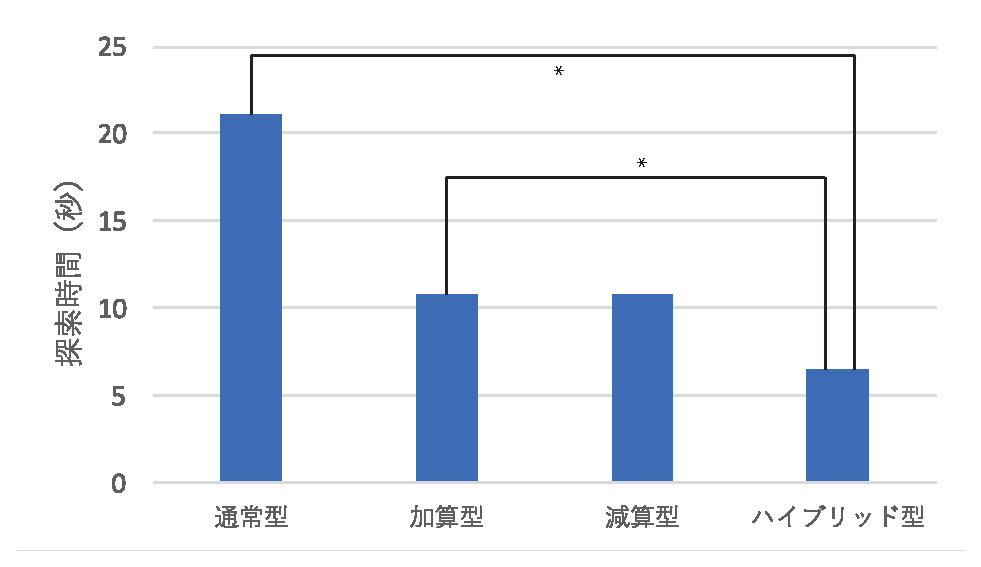
\includegraphics[clip, width=.95\textwidth]{dr_result1.eps}\\
          \small{(a)対象:単体}
        \end{minipage}
        \begin{minipage}{0.45\hsize}
          \centering
          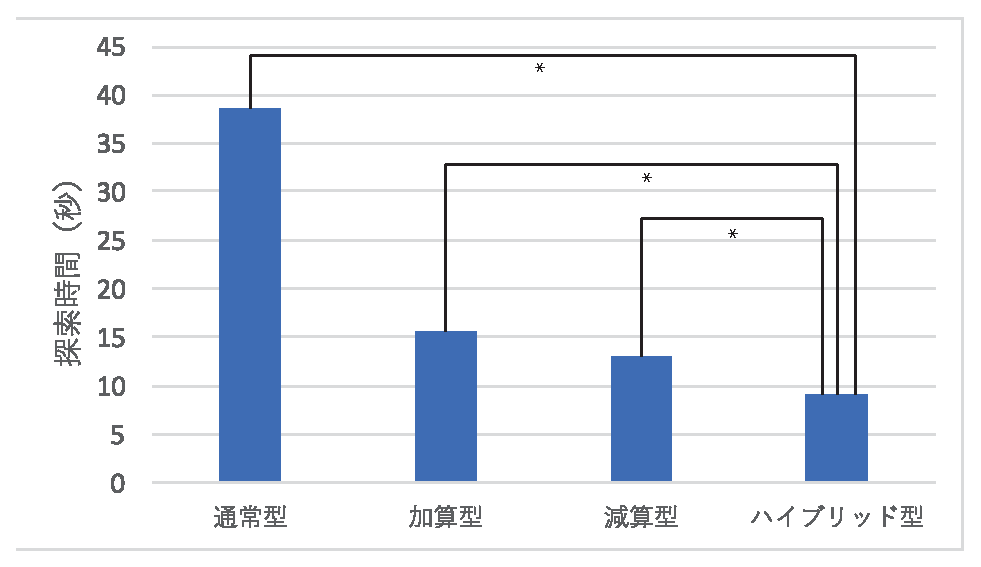
\includegraphics[clip, width=.95\textwidth]{dr_result2.eps}\\
          \small{(b)対象:複数}
        \end{minipage}
      \end{tabular}
      \vspace{2pt}
      \caption{実験結果:昼($*:p<.05$)(文献\cite{Kitamura:2017a}より図引用)}
      \label{figure:exp_dr_result_day}
      \vspace{2cm}
      \begin{tabular}{cc}
        \begin{minipage}{0.45\hsize}
          \centering
          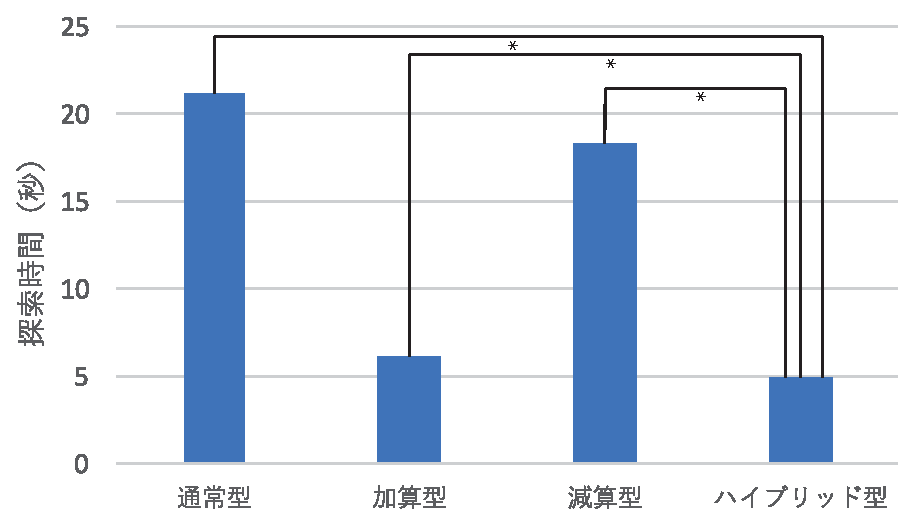
\includegraphics[clip, width=.95\textwidth]{dr_result3.eps}\\
          \small{(a)対象:単体}
        \end{minipage}
        \begin{minipage}{0.45\hsize}
          \centering
          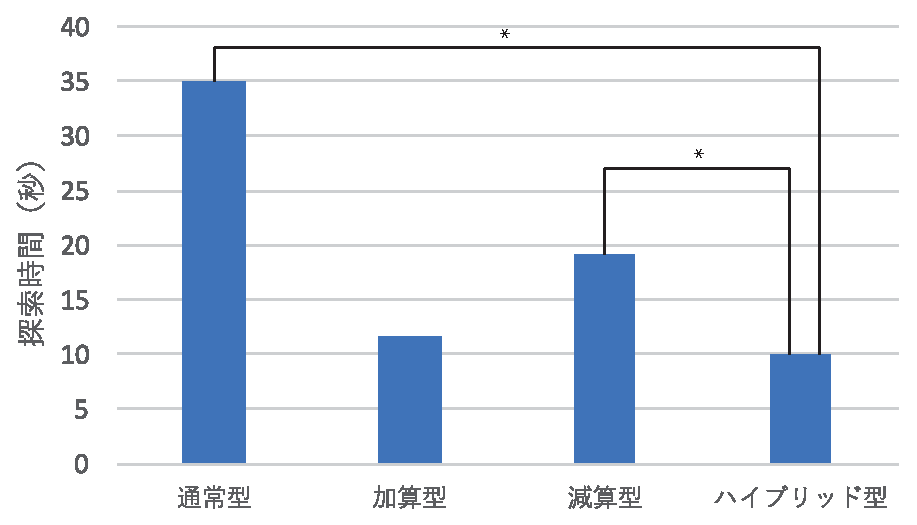
\includegraphics[clip, width=.95\textwidth]{dr_result4.eps}\\
          \small{(b)対象:複数}
        \end{minipage}
      \end{tabular}
      \vspace{2pt}
      \caption{実験結果:夜($*:p<.05$)(文献\cite{Kitamura:2017a}より図引用)}
      \label{figure:exp_dr_result_night}
    \end{center}
  \end{figure}
\chapter{看板認識に関する評価実験}

\section{実験の目的}

\section{実験の概要}

\section{実験の手続き}

\section{実験の結果}

\section{考察}
\chapter{Search by Snapを用いたユーザ実験}
\label{chapter:experiment_sbs}
本章では,Search by Snapを用いて実施したユーザ実験と,その結果について述べる.
\section{実験の目的}
  \ref{section:searching_action}節で述べたように,慣れていない地域や周囲の文字が読めない状況において,ユーザが目の前にある店舗の情報や条件に合致する店舗の情報を瞬時に取得することは容易ではない.
  位置情報を手がかりに周囲の検索を行い,条件に合った店舗が見つかったとしても,ユーザ自身が居る環境と検索行為とが分断されているため,ユーザの現在時点から検索対象の店舗を探す手間が残るという問題点がある.
  そのため,提案システムを用いることによって,位置情報を利用したサービスと比較して店舗を簡単かつ直感的に探索できることを確認する.
  本稿では,地域に慣れていないユーザを対象に評価を行う前段階として,提案システムのユーザビリティを評価するために,地元の大学生を対象にユーザ実験を実施する.

\section{予備実験}
  \subsection{実験の概要}
    実験は大阪府高槻市にある高槻本通りにおいて,\ref{chapter:implement_sbs}章で実装したシステムを用いて店舗を探索する際のユーザの行動を観察するために,ユーザが商店街において条件に合う店舗を探している状況を想定して行った.
    実験参加者は情報系の学部に通う大学生4名である.
    実験は昼間に行い,天候は曇りであった.

    表\ref{table:storelist}に示す15店舗を対象とし,実験参加者にはタスク(1)として,支払いにVISAカードが使える店舗を探すこと,タスク(2)として,月曜日の24時以降に営業している店舗を探すこと,の2点を課した.
    それぞれ提案システムを用いた場合とWeb検索エンジンを用いた場合とで探索に要した時間及び正確さを測定した.
    Web検索エンジンには,World Wide Web上で最も多く使われている検索エンジン\cite{Alexa:2019}であるGoogle検索\footnote{\url{https://www.google.com}(2019/2/1存在確認)}を用いる.
    実験に用いる端末は\ref{chapter:experiment_dr}章と同じNexus 7である.
    
  \subsection{実験の手順}
    探索に用いる手法の順序効果によるデータの偏りを排除するため,実験は2人同時に行い,タスク(1)は1人が提案システムを用いて行い,もう1人がGoogle検索を用いて行う.
    2人がタスク(1)を終えたら,実験参加者はタスク(2)を異なる手法を用いて行う.

    実験の手順として,初めに,実験参加者に回答用フォームのURLを伝え,参加者は自身のスマートフォンでフォームを開く.
    次に,提案システムの操作方法を実験参加者に説明する.
    その後,2人の実験参加者が同時に探索を開始し,フォーム上で条件に合致する店舗のチェックボックスを選択する.
    実験参加者が探索を開始してから送信ボタンをタップするまでの時間を測定する.
    
    実験終了後には,参加者に「求めていた情報の見つけやすさ(簡便性)」,「情報探索の直感性(直感性)」について,提案システムとGoogle検索との間で5段階のリッカート尺度を用い,「1」を「Google検索」,「5」を「提案システム」として5段階評価のアンケートへの回答を求めた.

  \subsection{実験の結果と考察}
    実験の結果を図\ref{figure:exp_sbs_pre_result_time},\ref{figure:exp_sbs_pre_result_acc}に示す.
    探索時間に関して,システムを用いた場合の探索時間はGoogle検索を用いた場合と比較して短くなる傾向が見られた.
    正確さに関して,システムを用いた場合の正確性はGoogle検索を用いた場合とで差が見られない傾向があった.
    アンケートの結果を表\ref{table:exp_sbs_pre_questionnaire}に示す.
    アンケートの結果から,提案システムを用いることによって,Google検索を用いた場合より直感的かつ簡易に探索ができるようになることが示唆された.

    \begin{figure}[tb]
      \begin{center}
        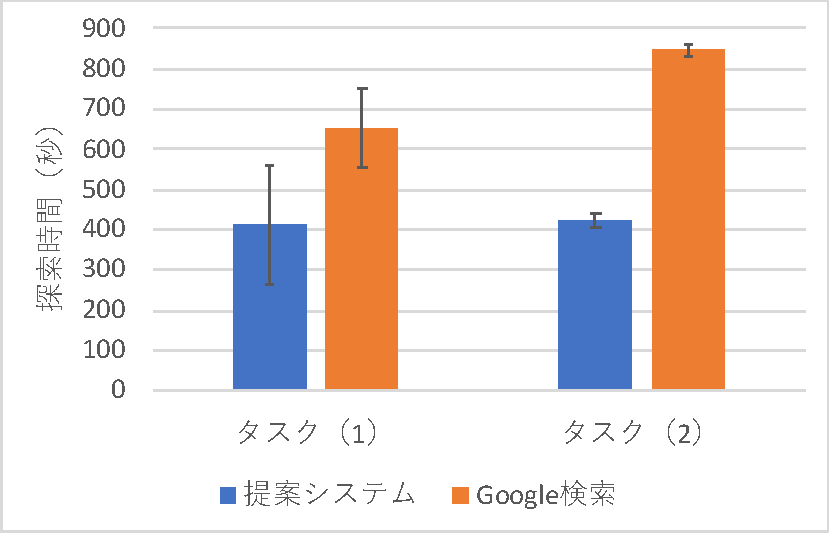
\includegraphics[clip, width=.95\columnwidth]{sbs_pre_result_time.pdf}
        \caption{予備実験の結果(探索時間)}
        \label{figure:exp_sbs_pre_result_time}
      \end{center}
    \end{figure}
    \begin{figure}[tb]
      \begin{center}
        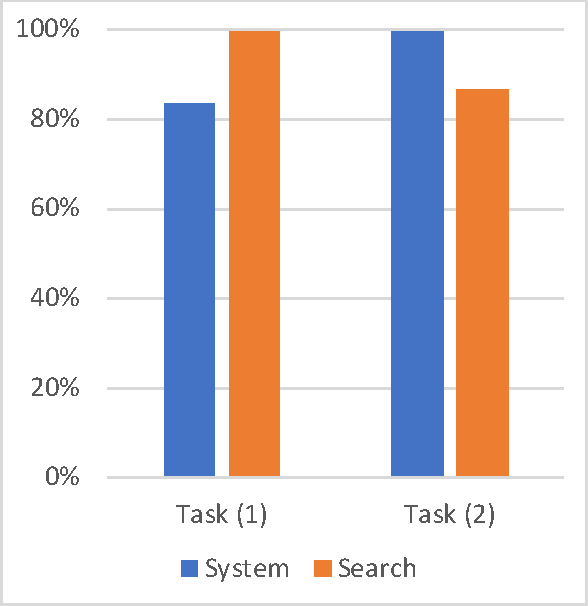
\includegraphics[clip, width=.95\columnwidth]{sbs_pre_result_acc.pdf}
        \caption{予備実験の結果(正解率)}
        \label{figure:exp_sbs_pre_result_acc}
      \end{center}
    \end{figure}

    \begin{table}
      \begin{center}
        \caption{予備実験のアンケート結果}
        \label{table:exp_sbs_pre_questionnaire}
        \begin{tabular}{c|ccp{9cm}}
          \hline \hline
          \textbf{実験参加者} & \textbf{簡便性} & \textbf{直感性} & \multicolumn{1}{c}{\textbf{コメント}} \\
          \hline
          A & 5 & 5 & カメラを向けるだけですぐ情報が見えるのでよかった \\
          B & 5 & 5 & 看板を映してパッと求めている情報が出てくるのはとても良いなと思いました。情報が見つけやすい。 \\
          C & 4 & 5 & 同じ地域に何店舗もある店だと検索サイトで検索した際、どの店かわかりづらく時間がかかりました。 \\
          D & 5 & 4 & \\
          \hline
        \end{tabular}
      \end{center}
    \end{table}

  \subsection{ユーザ観察}
    実験中のユーザを観察した結果,システムを用いて探索する際,至近距離で看板を認識しようとする行動が見られた.端末のカメラが店舗の看板の大部分の領域を捉えられない場合,正常に看板を認識できない場合が多いため,本実験では看板から一定の距離を置いて端末のカメラを向けるよう指示を与える.Google検索を用いて探索する際,多くのユーザがタスク(1)においては「(店舗名) 高槻」というクエリ,タスク(2)においては「(店舗名) 高槻 営業時間」というクエリで検索を行っていた.対象がチェーン店である場合,位置に関する情報をクエリとして与えなければ目的の情報に素早く辿り着けず,探索に時間を要している傾向が見られた.多くのユーザは,対象が飲食店である場合において,Google検索結果に表示された食べログのサイトへ移動し,そこから情報を得ていた.そのため,本実験では,探索対象を飲食店に限定し,食べログを用いて提案システムとの比較を行う.

\section{本実験}
  \subsection{実験の概要}
    実験は大阪府高槻市にある高槻本通りにおいて,昼間にユーザが飲食店を探している状況を想定して行った.
    実験参加者は情報系の学部に通う大学生10名である.

    実験参加者にはタスク(A)として,「小だるま JR高槻駅前店」,「肉丼専門店 高槻肉劇場」,「磯丸水産 高槻店」の3店舗について,使用できるクレジットカードの種類を``Visa'',``Mastercard'',``JCB'',``American Express'',``Diners Club''の5つのチェックボックスから全て選択すること,タスク(B)として,「おだいどこはなれ 高槻店」,「高槻ちゃぶちゃぶ」,「赤から 高槻店」の3店舗について,月曜日の営業開始時刻を数値で入力すること,の2点を課した.
    タスク(A)は図\ref{figure:exp_sbs_point}中\textcircled{\scriptsize 1}で示した位置に立った状態,タスク(B)は図\ref{figure:exp_sbs_point}中\textcircled{\scriptsize 2}で示した位置に立った状態で行った.
    実験に用いた携帯端末はクアンタ・コンピュータ社\footnote{\url{http://www.quantatw.com}(2019/2/8存在確認)}のVA-10J(Android 5.0.2)である.
    提案システムとの比較対象とする位置情報を用いたサービスは,ランキングやユーザの口コミ・写真をもとにレストランの検索が行えるサービスである食べログ\footnote{\url{https://tabelog.com}(2019/2/8存在確認)}を用いた.

  \begin{figure}[tb]
    \begin{center}
      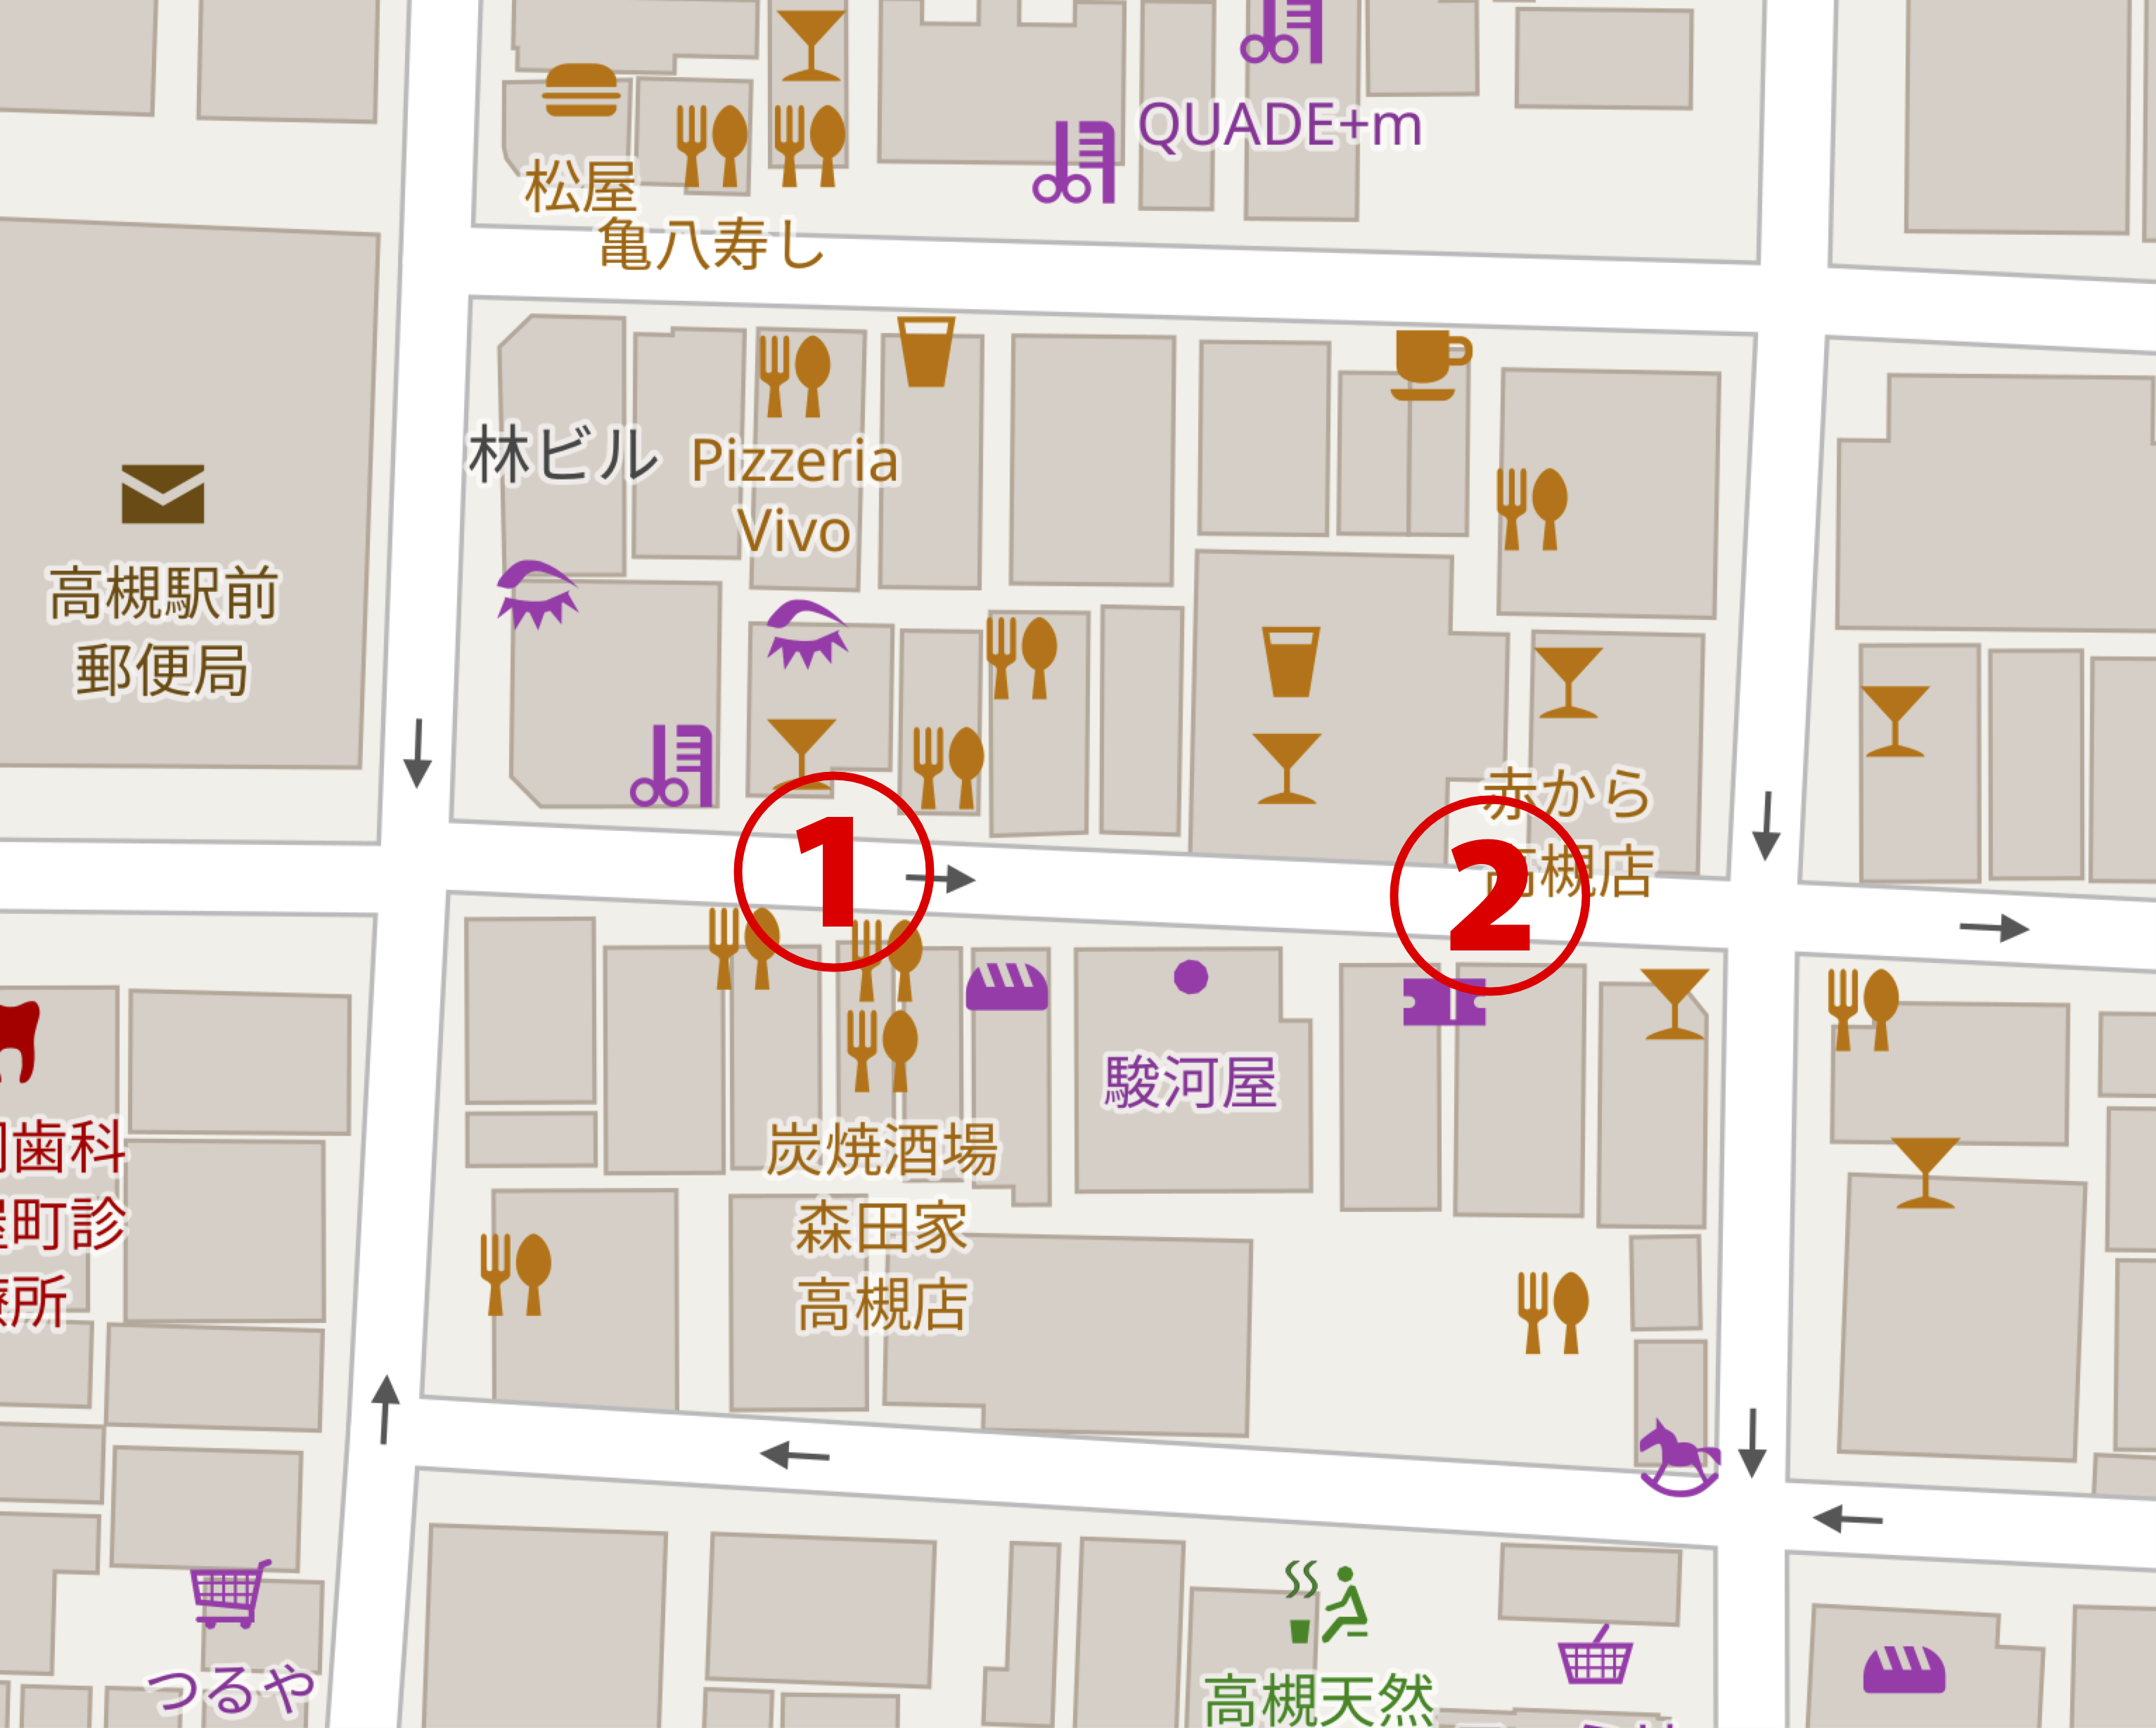
\includegraphics[clip, width=.95\columnwidth]{sbs_map_point.png}
      \caption{実験の実施地点}
      \label{figure:exp_sbs_point}
    \end{center}
  \end{figure}

  \begin{figure}[tb]
    \centerline{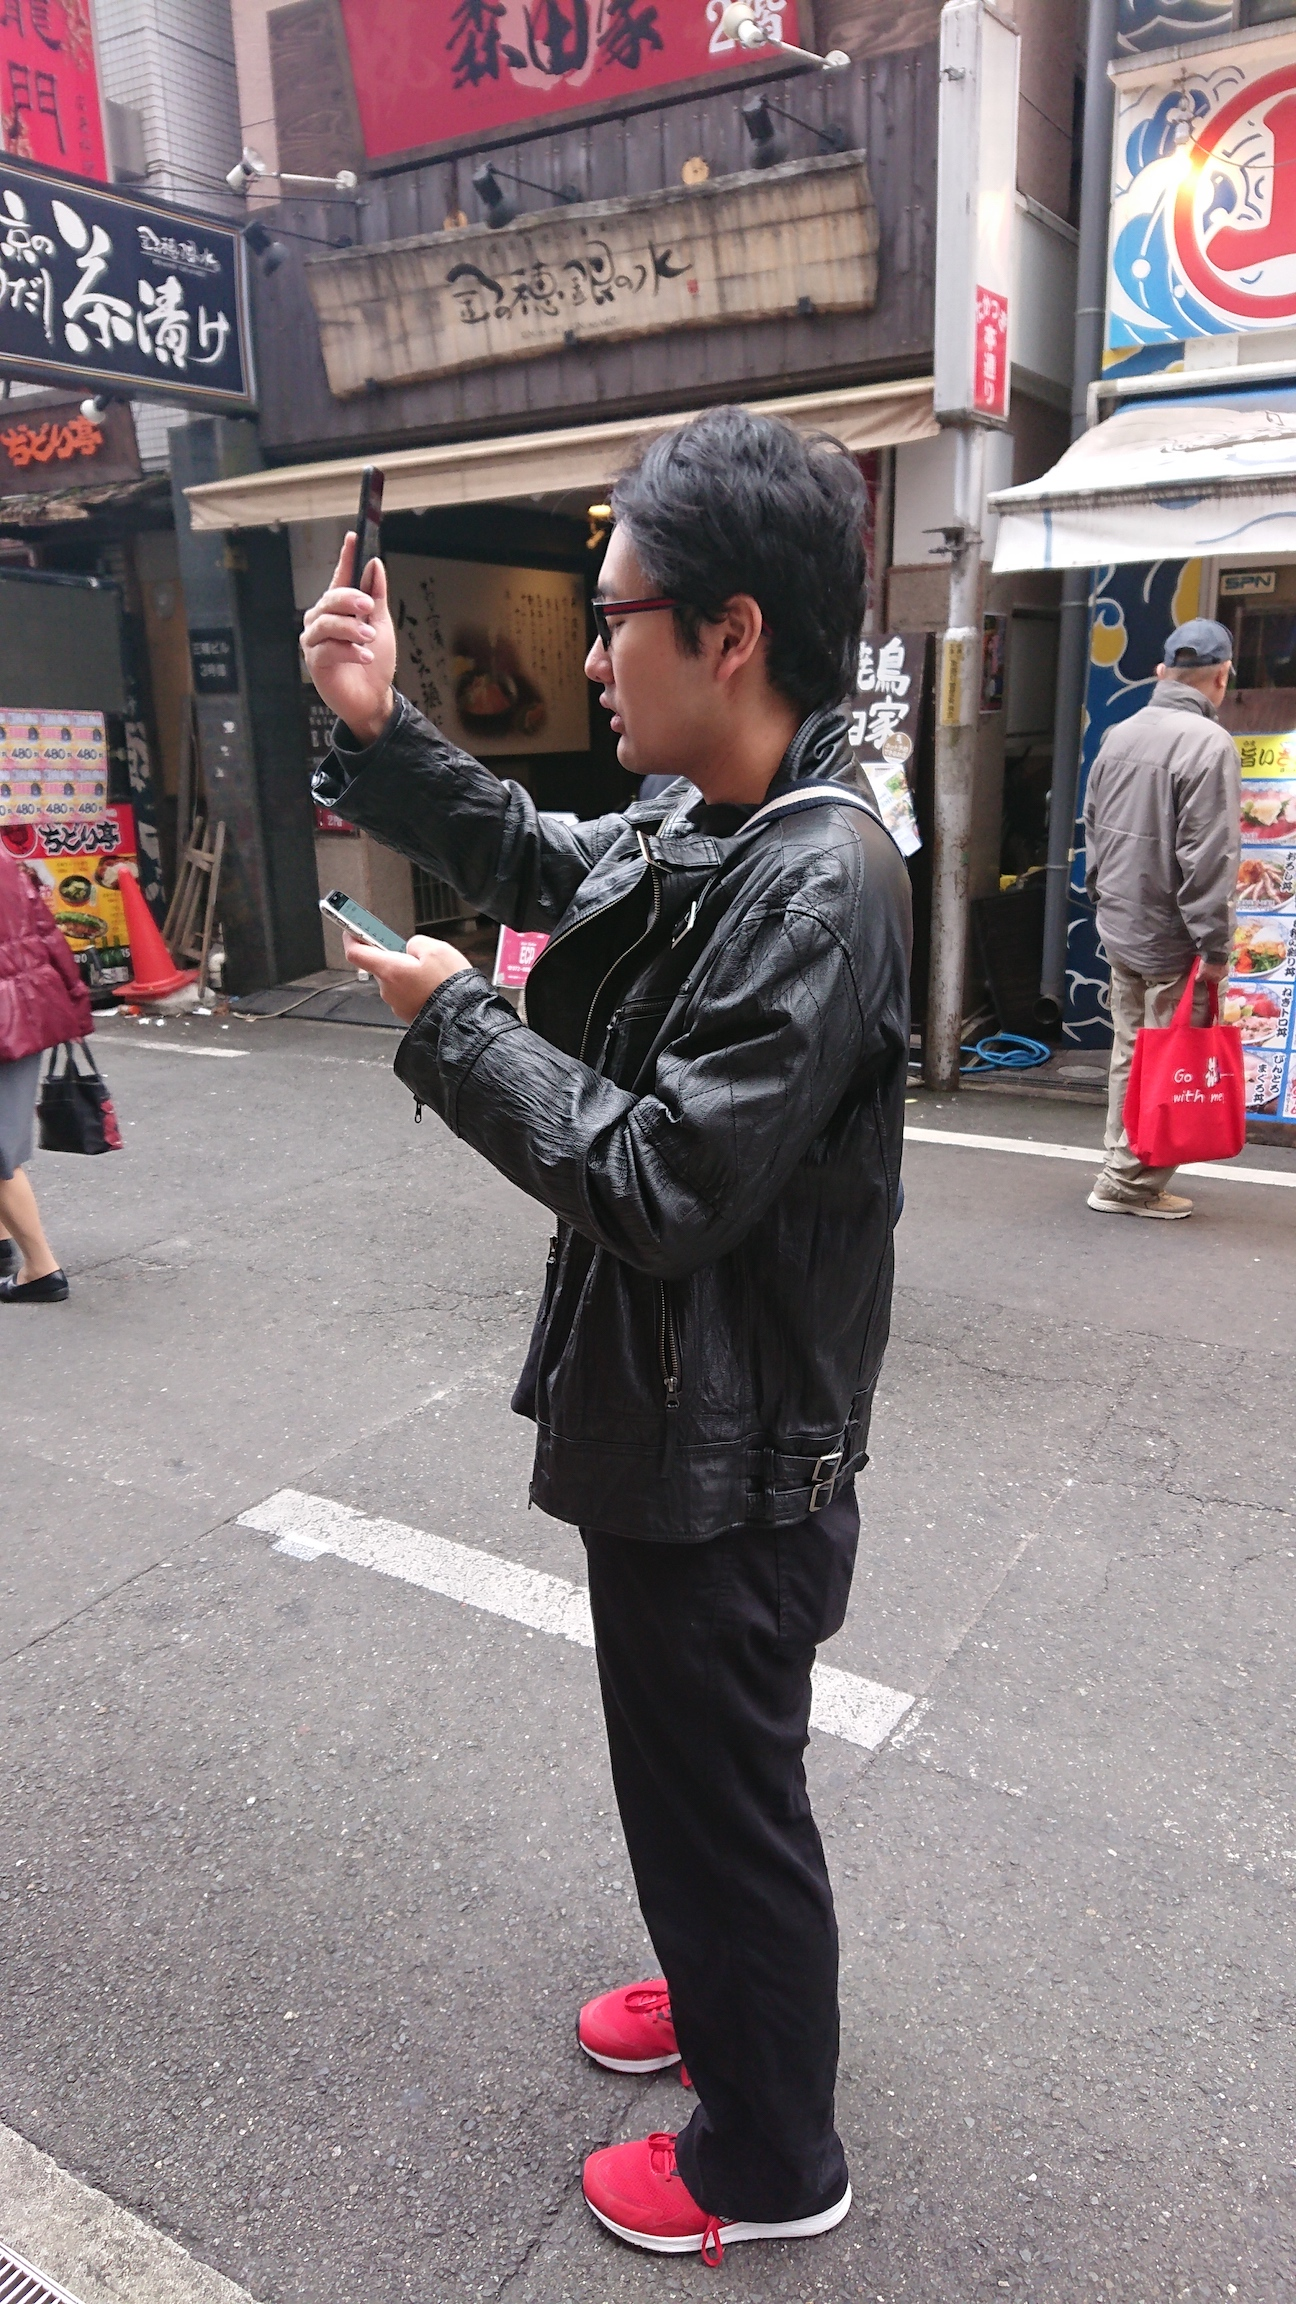
\includegraphics[width=.5\columnwidth, clip]{sbs_exp_scenery.jpg}}
    \caption{実験の風景}
    \label{figure:exp_sbs_scenery}
  \end{figure}

  \subsection{実験の手順}
    初めに,提案システムと食べログの使い方を実験参加者に説明する.
    次に,実験参加者に回答用フォームのURLを伝え,参加者は自身のスマートフォンでフォームを開く.
    実験に用いるシステムを起動した状態で参加者に実験用のスマートフォンを渡す.
    実験参加者はシステムを用いて求められている情報を探索し,フォームに入力して送信する.
    実験参加者がシステムの操作を始めてから送信ボタンをタップするまでの時間を計測する.
    実験の風景を図\ref{figure:exp_sbs_scenery}に示す.

    実験参加者をグループ(1)とグループ(2)に2分割し,グループ(1)にはタスク(A)を提案システム,タスク(B)を食べログを用いて行うよう指示を出し,グループ(2)にはタスク(A)を食べログ,タスク(B)を提案システムを用いて行うよう指示を出した.
    実験終了後には,参加者に「求めていた情報の見つけやすさ(簡便性)」,「情報探索の直感性(直感性)」について,食べログと提案システムとの間で5段階評価のアンケートへの回答を求めた.

  \subsection{実験の結果}
    実験参加者がシステムに操作を初めてから指示された情報を全て収集し,送信ボタンをタップするまでの時間を計測し,タスク(A)とタスク(B)に関して提案システムを用いた場合と食べログを用いた場合とにおいて,探索時間の平均値を比較した.その結果を図\ref{figure:exp_sbs_result_time}に示す.
    タスク(A)において,提案手法を用いた場合の探索時間は食べログを用いた場合よりも有意に短い($t(8)=2.343, p<.05$)ことが確認された.
    タスク(B)においても,提案手法を用いた場合の探索時間は食べログを用いた場合よりも有意に短い($t(8)=4.370, p<.05$)ことが確認された.

    各タスクにおいて,ユーザが正確に情報を収集できたかを測定するために,対象とした3店舗のうち,正確に情報を取得できた店舗数の割合を正解率として測定し,提案システムを用いた場合と食べログを用いた場合とにおいて,正解率の平均値を比較した.その結果を図\ref{figure:exp_sbs_result_acc}に示す.
    タスク(A)において,提案手法を用いた場合と食べログを用いた場合とで,正解率に有意差は見られなかった($t(8)=1.000, n.s.$).
    タスク(B)においても,提案手法を用いた場合と食べログを用いた場合とで,正解率に有意差は見られなかった($t(8)=1.633, n.s.$).

    予備実験と同様に,実験終了後に情報探索の簡便性と直感性について5段階のリッカート尺度を用い,「1」を「食べログ」,「5」を「提案システム」として5段階で回答してもらった.
    簡便性に関する平均値は4.4,直感性に関する平均値は4.5であった.
    そのアンケート結果を表\ref{table:exp_sbs_questionnaire}に,アンケート結果の分布を図\ref{figure:exp_sbs_result_question}に示す.
    
    \begin{figure}[tb]
      \begin{center}
        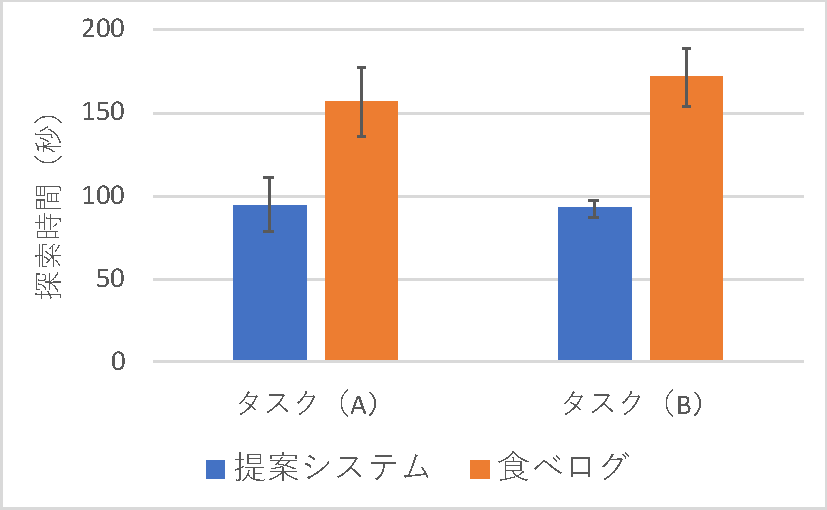
\includegraphics[clip, width=.95\columnwidth]{sbs_result_time.pdf}
        \caption{本実験の結果(探索時間)}
        \label{figure:exp_sbs_result_time}
      \end{center}
      \vspace{1cm}
      \begin{center}
        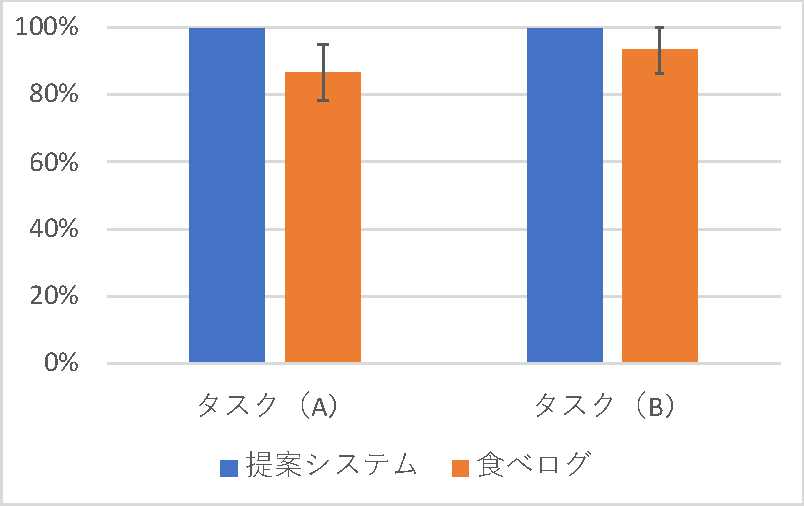
\includegraphics[clip, width=.95\columnwidth]{sbs_result_acc.pdf}
        \caption{本実験の結果(正解率)}
        \label{figure:exp_sbs_result_acc}
      \end{center}
    \end{figure}

    \begin{table}
      \begin{center}
        \caption{本実験のアンケート結果}
        \label{table:exp_sbs_questionnaire}
        \begin{tabular}{c|cccp{8cm}}
          \hline \hline
          \textbf{実験参加者} & \textbf{群} & \textbf{簡便性} & \textbf{直感性} & \multicolumn{1}{c}{\textbf{コメント}} \\
          \hline
          1  & A & 5 & 5 & 看板が多いところだと情報の表示が重なり見にくいところがあった。 \\
          2  & A & 4 & 4 & どちらの検索機能も分かりやすいと思います。 \\
          3  & A & 5 & 5 & リアルタイムな情報が検索できたらもっと便利かと思いました。 \\
          4  & A & 2 & 4 & システムを使った時に店の情報が違う店の情報に被ってしまって見にくいときがあったことと、情報が一定の場所に出続けないてなくて毎回情報と、店名とを見比べる必要がありました \\
          5  & A & 4 & 4 & 食べログはUI次第でどうにかなると思いました。 システムの方は、文字を色分けなどしていただいた方が目につきやすいのかとおもいました。 \\
          6  & B & 5 & 5 & タップ数やかかる時間でもシステムの方が有利に感じた。 \\
          7  & B & 5 & 4 & システムでは、欲しい店舗の情報を常に表示し続けるためには かざし続けなければいけなく、ズレてしまった場合 違う店舗情報が出てしまったため 慣れが必要なのかなと思いました。一方、食べログ検索では店舗によって載ってる情報がバラバラなため、必要な情報がなかった際に 本当に情報が無いのかのダブルチェックを必要とすることが億劫であった。 \\
          8  & B & 5 & 5 &  \\
          9  & B & 5 & 4 &  \\
          10 & B & 4 & 5 & すぐに情報を知れて便利だと思いました。 \\
          \hline
        \end{tabular}
      \end{center}
    \end{table}    

    \begin{figure}[tb]
      \begin{center}
        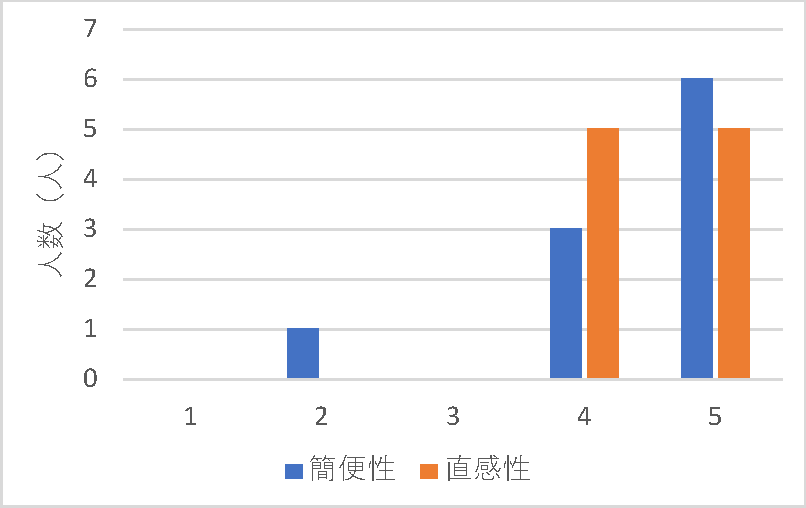
\includegraphics[clip, width=.95\columnwidth]{sbs_result_question.pdf}
        \caption{本実験のアンケート結果の分布(1: 食べログ〜 5: 提案システム)}
        \label{figure:exp_sbs_result_question}
      \end{center}
    \end{figure}
\chapter{議論}
\label{chapter:discussion}
本章では,\ref{chapter:experiment_dr}章と\ref{chapter:experiment_sbs}章で述べた実験の結果に基づき,本研究の到達点と改善点,今後の展望について述べる.

\section{得られた知見}
\label{section:obtained_knowledge}
  \ref{chapter:experiment_dr}章で述べた実験では,探索対象が単体であり,時間帯が昼の場合,提案手法であるハイブリッド型情報提示手法は文献\cite{Fujita:2013}で提案された減算型情報提示手法と探索時間に関して有意差は見られなかった.しかし,探索対象が複数の場合及び時間帯が夜で探索対象が単体の場合においては,提案手法は減算型情報提示手法よりも探索時間が有意に短いことが確認された.このことから,背景の彩度が低い場合や複数の看板を探索する場合において,提案手法は有効であると考えられる.また,時間帯が夜で探索対象が複数である場合,加算型情報提示手法と比較して減算型情報提示手法の方が探索時間が長くなる傾向が見られた.これは実験に用いた写真の背景の彩度が低かったこと,新日本新地ビルの看板に白と黒から構成されているものが多く含まれていたことにより,減算の効果が減少したことが原因と考えられる.

  \ref{chapter:experiment_sbs}章で行なった実験の結果から,情報探索時間に関しては,本稿で扱ったいずれの場合においても,提案システムを用いた場合は食べログを用いた場合よりも探索時間が有意に短くなることが明らかとなった.このことから,提案システムを用いることによって,位置情報のみを用いた場合と比較してユーザはより素早く求めている情報を取得することが可能になるといえる.
  情報探索の正確さに関しては,本稿で扱ったいずれの場合においても,提案システムを用いた場合と食べログを用いた場合とでは正解率に有意差は見られなかった.このことから,言語障壁がなければ位置情報のみを用いても正確に情報を探索することが可能であり,提案システムを用いた場合においても正確な情報探索が可能であるといえる.
  さらに,アンケート結果から,提案システムを用いることによって,位置情報のみを用いた場合と比較してより簡単かつ直感的に情報が探索できるようになることが示唆された.

\section{本研究の到達点}
  \ref{chapter:experiment_dr}章で実施した実験では,文献\cite{Fujita:2013}で提案された減算型情報提示手法に文字情報を追加した加算型と減算型のハイブリッド型情報提示手法を提案した.提案手法を用いたシステムのプロトタイプを実装することにより,減算型情報提示手法の問題点であった,不要な情報を減算する際に対象となる看板が白黒であり,かつその周辺の景色の彩度が低い場合に減算の効果が減少するという点が解消されたと考えられる.これにより,彩度が低い環境においても分かりやすい情報提示が可能となった.また,実験結果から看板を探索する際,提案手法を用いることによって探索時間が短くなることが確認された.以上により,\ref{section:purpose}節で述べた看板密集地域における視覚情報の識別性の向上,及び探索時間の短縮が可能になった.

  提案システムを用いることによって,本研究の目的である,ユーザの目の前にある店舗の情報を直感的かつ簡単に取得できることが達成されたと考えられる.
  これにより,?章で述べた,慣れていない地域においても,ユーザが求める条件に合致する店舗を探索できるようになることが示唆された.

\section{改善点}
  \subsection{減算型表示の実環境における実験}
    \ref{chapter:implement_dr}章で実装したシステムは特定の位置で撮影した全天球画像内でのみ店舗の探索が行えるため,\ref{chapter:experiment_dr}章で実施した実験は,人工環境内のみである.そのため,実環境においても本稿で提案した情報提示手法が有用であるかを検証する必要がある.\ref{chapter:implement_recog}章で実装したリアルタイム看板認識APIを用いることにより,実環境での実験が可能になるため,看板が密集している地域においてOSMのデータベースと看板データベースを構築し,実環境において提案手法の優位性を検討する.

  \subsection{看板認識手法}
    \ref{chapter:implement_recog}章で実装したシステムの改善点として,(1)OSMのノードと看板画像を手作業で関連付けなければならない点,(2)インターネット上の情報から多種多様な店舗の看板画像を大量に集めることは困難であるため,手作業で看板画像を1店舗につき100枚程度集めなければならない点,が挙げられる.
    (1)に対しては,看板画像を提示してユーザに店舗名を回答するシステムを実装することで解決でき,(2)に対してはユーザに店舗の看板画像を提示し,それと同じ写真を撮影して投稿するシステムを実装することで解決できると考えられる.
    これらのシステムにゲーミフィケーションを利用し,ユーザの行動に対して報酬を与えることによって,多数のデータを効率よく収集できると考えられる.
    
    今後の展望として,看板認識をサーバ上で行うのではなく,Tiny--YOLO等を用いて携帯端末上で行うことを検討する.これにより,サーバへ画像を送信する必要がなくなるため,通信量の大幅な軽減が期待される.

  \subsection{対象地域の拡張}
    \ref{chapter:experiment_sbs}章で
    OSMのデータは誰もが編集可能であるため,その地域に慣れている地元のユーザが自身でデータを収集し,OSMを通して活用できるようになる枠組みの構築を目指す.
    OSMのノードには``cuisine''タグが存在し,``burger'',``noodle'',``japanese'',``chinese''など,飲食店で提供される食品の種類を表す値を追加できる.他にもベジタリアン向けのメニューが提供されていることを表す``diet:vegetarian''や,イスラム教の戒律で許されている食品のみを使用したメニューが提供されていることを表す``diet:halal''などのタグも存在する.
    さらに,店舗名の英語またはローマ字表記を表す``name:en''タグや中国語表記の``name:zh''タグ,韓国語表記の``name:ko''タグなどを充実させることによって,ユーザインタフェースを多言語に対応させることが可能となる.
    これらのデータを活用することにより,その地域に慣れていない人や,地元の文字が読めない外国人観光客に対して,求めている情報を容易に取得でき,アレルギーや宗教的制約などの理由による食事制限にも対応可能なナビゲーションを実現できる.
    
    本稿における実験参加者は地元の大学生であるため,地域に慣れていないユーザや非漢字圏など地元の文字が読めないユーザを対象としたユーザ実験を実施する.
\chapter{結論}
\label{chapter:conclusion}
  本研究の目的は,ユーザが慣れていない地域や周囲の文字が読めない状況であっても,目の前にある店舗の情報を直感的かつ簡便に取得できるシステムの実現である.
  本稿では「周囲に看板が多数存在する状況」と「周囲の文字が読めない状況」を対象としたプロトタイプを実装し,ユーザ実験を行うことで,既存のシステムとの差異を明らかにした.
  以下の本稿の内容を纏める.

  \ref{chapter:introduction}章では,本研究に至った背景と問題点を述べ,解決すべき課題を明らかにした.
  街中における店舗の看板は,人々が求める条件に合致した店舗を探す際に重要な役割を果たしている.
  しかし,街中における情報探索の問題点として(1)繁華街など看板が密集している地域においては,大量に存在する他の視覚情報に紛れて目的の看板を見つけることが出来ない可能性があること,(2)外国人観光客の場合,言語障壁により目の前にある店舗が自身の求める条件に合致するか検索することが困難である点,の2点を挙げた.
  (1)に対しては,ユーザにとって不要な情報を目立たなくさせ,必要な情報には追加情報を重畳表示すること,(2)に対しては,スマートフォンのカメラを通して店舗の看板を見るとカメラ映像上に店舗の詳細情報が得られるシステムを実装することにより,これらの問題を解決すると述べた.
  これらの提案手法の優位性を検証するために,従来手法と比較したユーザ実験を行うことを述べた.

  \ref{chapter:relatedwork}章では,本研究で提案するシステムの実現に関連する研究を述べ,本研究の位置付けを明らかにした.
  まず,ARを用いたナビゲーションシステムについて説明し,ARを用いることで紙の地図を用いる場合と比較してより少ない時間で目的地まで辿り着けることについて述べた.
  次に,情報の視認性に関する研究として,解像度制御による視線誘導と,隠消現実感について述べた.
  続いて,看板認識に関する研究として,OCRを用いて看板に描かれている文字を認識する研究や,物体検出に関する研究として,CNNを用いて画像の中から物体領域を検出する研究について述べた.
  最後に,本研究の位置付けとして,Vision-based ARを用いることと,CNNを用いて看板を認識することを述べた.

  \ref{chapter:design_guidline}章では,これまでの取り組みとして,減算型表示について説明し,本研究で対象とする状況及び提案システムの要件について述べた.
  加えて,提案システムの要件を満たすための前提条件と,本稿の提案手法であるSearch by Snapについて説明し,そのインタフェースのデザインについて述べた.

  \ref{chapter:implement_dr}章では,減算型表示を用いたプロトタイプの実装について述べた.
  プロトタイプでは,ユーザはモバイルデバイスを全天球画像内で全方向に向けることができ,選択されていない種類の店舗の視覚情報を減算すると述べた.

  \ref{chapter:implement_recog}章では,リアルタイムで看板認識を行うために実装したAPIについて述べた.
  (1)YOLOv2を用いて看板領域を検出し,(2)VGG16を用いて看板を分類することにより,画像内の看板を認識することを述べた.
  リアルタイムで看板認識を行うために,GPUを搭載したマシン上にWeb APIサーバを構築し,モバイルデバイスからAPIを呼び出すことでリアルタイム認識を実現した.

  \ref{chapter:implement_sbs}章では,\ref{chapter:design_guidline}章で述べたデザイン指針に基づき,Search by Snapを用いて実装したプロトタイプについて述べた.
  \ref{chapter:implement_recog}章で実装したAPIと,OpenStreetMapのデータベースに格納されている店舗情報を用いることによって,ユーザがモバイルデバイスのカメラを通して店舗の看板を見ると,その店舗の情報が得られるシステムを実装した.

  \ref{chapter:experiment_dr}章では,\ref{chapter:implement_dr}章で実装したプロトタイプを用いて実施した評価実験について述べた.
  実験参加者には,全天球画像内で指示された看板を探索するタスクを課した.
  実験の結果,ユーザにとって不要な視覚情報を減算し,必要な情報には付加情報を重畳表示することによって,探索時間が有意に短くなることを示した.

  \ref{chapter:experiment_sbs}章では,\ref{chapter:implement_sbs}章で実装したプロトタイプを用いて実施したユーザ実験について述べた.
  実験参加者には,実際の商店街において,ユーザが条件に合う店舗を探している状況を想定し,使えるクレジットカードの種類と月曜日の営業開始時刻を調べるタスクを課した.
  提案システムと位置情報を用いた検索サービスとを比較した結果,探索時間に関しては提案システムを用いることで有意に短くなることを示し,正解率に関しては有意差がなく,どちらも正確に探索ができることを示した.

  \ref{chapter:discussion}章では,\ref{chapter:experiment_dr}章及び\ref{chapter:experiment_sbs}章で実施した実験から得られた知見と本研究の到達点,提案システムの改善点を述べた.
  本稿で提案した2つのシステムを用いることによって,ユーザが慣れていない地域においても,ユーザが求める条件に合致する店舗を探索できるようになることが示唆された.
  改善点としては,(1)\ref{chapter:implement_dr}で実装したプロトタイプを実環境でも利用できるよう新たに実装を行う点,(2)看板認識に必要なデータセットを効率よく収集する手法を確立する点,(3)OSMのデータベースの充実やインタフェースを多言語化する点,の3点が挙げられる.

  \ref{chapter:conclusion}章では,本稿の要点をまとめ結論づけた.
\chapter*{謝辞}
全ての人と馬に感謝いたします.

\bibliographystyle{ipsjsort}
\bibliography{reference}


\end{document}